% Companion to main_prr.tex. The PRL supplement is preserved separately.
\documentclass[aps,10pt,onecolumn,superscriptaddress,nofootinbib,
  longbibliography,amsmath,amssymb,floatfix]{revtex4-2}
\usepackage[T1]{fontenc}
\usepackage{graphicx}
\usepackage{placeins}
\usepackage{hyperref}
\hypersetup{hidelinks}
\makeatletter
\AtBeginDocument{\immediate\write\@auxout{\string\citation{apsrev42Control}}}
\makeatother
\brokenpenalty=10000
\renewcommand{\thesection}{S\arabic{section}}
\renewcommand{\thefigure}{S\arabic{figure}}
\renewcommand{\thetable}{S\arabic{table}}
\renewcommand{\theequation}{S\arabic{equation}}
\newcommand{\Tr}{\operatorname{tr}}
\newcommand{\dd}{\mathrm{d}}

\begin{document}
\title{Supplemental Material for\texorpdfstring{\\}{: }
The Stronger Route Can Be the Worse Readout: Flexible Routing under a Fluctuation Budget}
\author{Mingyi Huang}
\noaffiliation
\author{Yuguo Yu}
\email{yuyuguo@fudan.edu.cn}
\noaffiliation
\maketitle

The main text asks what makes flexible routing useful to a receiver
with a prescribed temporal integration rule. Sections~\ref{sec:cost}--\ref{sec:crosssupp}
derive the cost laws, report full window-wise discrimination,
and prove why the budget price of a given reliability depends
on the output timescale. They also give the sensitivity tests
for the readout-ranking reversal. Section~\ref{sec:modularsupp}
derives the modular extension, local-noise endpoint test and
task-dependent allocation rules, and compares constrained readouts
with an optimal temporal decoder. Sections~\ref{sec:fly}--\ref{sec:allen}
then place the models beside connectome and recording analyses:
imposed gain on FlyWire anatomy, recovery after ALM perturbations,
and state-specific prediction in Allen visual recordings. These
extensions retain their individual statistical interpretations;
they do not establish biological budget optimization.
Section~\ref{sec:feedbacksupp} analyzes a budget-conserving
controller and tests it with finite decision feedback.
Section~\ref{sec:localgainsupp} lets neighboring routes exchange
target budgets and adjusts the gains using activity-based cost estimates.

\section{Extensions and scope of the stationary cost}
\label{sec:cost}

\subsection{Why the square-zero cost is quadratic}

Let \(J=-aI+\epsilon K\), where \(a>0\) is the common decay rate,
\(\epsilon\) scales the coupling, and \(K^m\ne0\) but \(K^{m+1}=0\).
Thus activity can pass through the coupling at most \(m\) times.
For isotropic white drive, the cost is the time integral of
\(e^{-2at}\|e^{\epsilon Kt}\|_F^2\). Expanding the finite exponential
polynomial and integrating gives
\begin{equation}
 C_I(J)=
 \sum_{j,l=0}^m
 \frac{(j+l)!\,\epsilon^{j+l}}{j!\,l!\,(2a)^{j+l+1}}
 \Tr\!\left[K^j(K^\top)^l\right].
 \label{eq:nilpotent}
\end{equation}
The degree-two coefficient is \(\|K\|_F^2/(4a^3)\), since
\(\Tr K^2=0\), and the linear coefficient vanishes. For \(m\ge2\), the
highest-degree coefficient is proportional to \(\|K^m\|_F^2>0\).
Consequently the cost \emph{as a function of coupling amplitude}
truncates at quadratic order exactly when \(K^2=0\), including \(K=0\).
Equality with the quadratic expression at an isolated parameter value
would not by itself imply this structural property.

The derivative of squared Euclidean response at \(t=0\) depends on
the symmetric part of \(J\), not directly on the integrated variance.
For example, a normalized three-node triangular coupling with all three
strictly upper-triangular entries \(1/\sqrt{3}\) has unit Frobenius
norm, and its symmetric part has largest eigenvalue \(1/\sqrt{3}\).
A unit-strength rank-one square-zero coupling gives \(1/2\).
Thus the triangle has a greater initial-growth slope per unit
Frobenius strength but pays additional variance costs at finite
coupling. The compared triangle and chain examples are numerical
tests at matched total cost, not an exhaustive search over directed
generators. Figure~\ref{fig:chains} shows the uniform-chain
comparisons at matched cost. Figure~\ref{fig:general}(a) checks the local quadratic
cost against the stationary covariance. Panel (b) shows where that
quadratic law ceases to describe the triangle as coupling increases;
the one-pass example stays on the law. Panel (c) compares the
resulting gains at the same cost.

\begin{figure}[t]
\centering
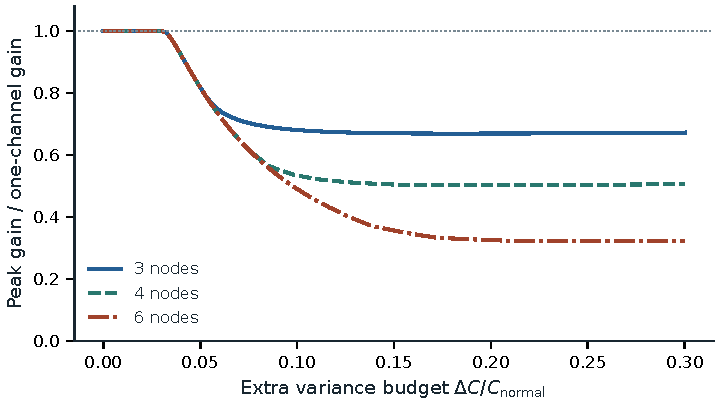
\includegraphics[width=0.60\textwidth]{figures/fig_prrS_chain.pdf}
\caption{\textbf{Uniform chains at the same variance cost as one channel.}
The ordinate divides each chain's peak squared gain by the
one-channel gain at the same cost. Each system uses \(N=64\),
equal decay \(a=0.2\), and independent unit drive. None of the
tested chains improves on one channel.}
\label{fig:chains}
\end{figure}

\begin{figure}[t]
\centering
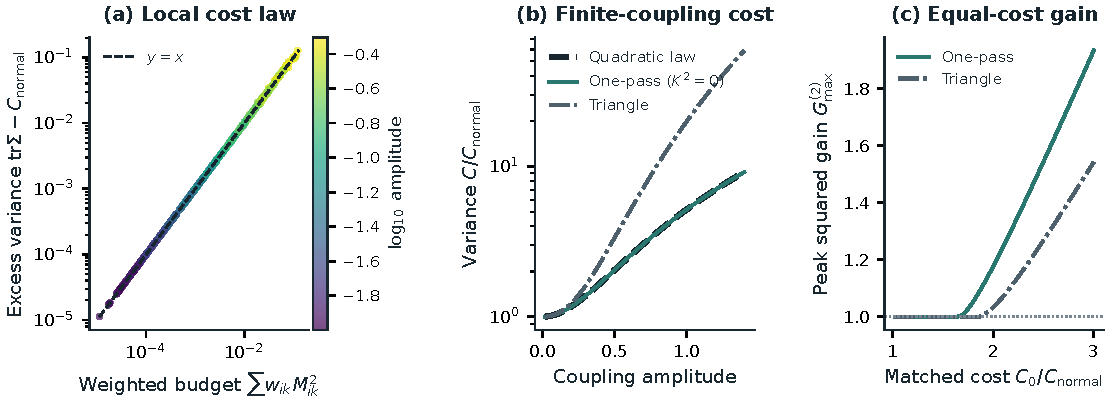
\includegraphics[width=\textwidth]{figures/fig_general_spectrum.pdf}
\caption{\textbf{Local real-spectrum law and finite-coupling checks.}
(a) The leading excess variance cost for stable real spectra approaches
the weighted quadratic expression at weak coupling.
(b) An isolated square-zero channel obeys that expression exactly,
while a triangle can depart from it.
(c) The displayed matched-cost comparisons are for selected coupling
families and do not imply a generic upper bound.}
\label{fig:general}
\end{figure}

\subsection{Numerical check of the target-gain cost}
For the isolated pair we evaluate the time minimization on a
logarithmic grid and refine the minimum. We independently check the
gain by the singular values of a dense matrix exponential and the
cost by a Lyapunov solve. This covers four decay pairs at squared
gain targets \(1.0001,1.2,2,4\). At \(G=2\) the decay pairs
\((0.20,0.20)\), \((0.10,0.30)\) and \((0.04,0.36)\) all have onset
cost \(5\), but target costs \(15.629\), \(17.925\) and \(27.019\),
respectively. The right-hand onset limit is checked separately.
At fixed \(a_i+a_k=0.4\), we also scanned 36 values of the fractional
rate mismatch \(|a_i-a_k|/(a_i+a_k)\) from \(0.01\) to \(0.99\) and 55
values of \(G-1\) from \(10^{-6}\) to \(10^3\), both logarithmically
spaced. None of the 1,980 unequal-rate cases costs less than the
equal-rate pair at the same \(G\). This scan does not establish a
minimum over all rate ratios and gains.

\subsection{Discrete-time one-pass couplings}
For a one-step map \(A=\rho I+K\) in \(N\) dimensions, assume
\(|\rho|<1\), \(K^2=0\), and unit isotropic drive per step. Then
\(A^k=\rho^k I+k\rho^{k-1}K\) for \(k\ge1\), interpreted at
\(\rho=0\) as \(A=K\), \(A^{k\ge2}=0\). Since \(\Tr K=0\), the
stationary variance is
\begin{equation}
 \sum_{k=0}^{\infty}\|A^k\|_F^2
 =\frac{N}{1-\rho^2}+
   \frac{1+\rho^2}{(1-\rho^2)^3}\|K\|_F^2.
\end{equation}
The second coefficient sums \(k^2\rho^{2(k-1)}\). At each step the
propagator norm is nondecreasing in the largest singular value of
\(K\): on each orthogonal source--target pair the diagonal has equal
magnitude and the off-diagonal has magnitude \(k|\rho|^{k-1}s_i\).
Thus rank-one allocation attains the maximum peak gain at fixed cost;
there need not be a unique allocation when the maximum is one.
This equal-decay identity is not a frontier for the heterogeneous
fitted operators below.

\subsection{Allocation with anisotropic drive and feasible channels}

Write \(K=\sum_i s_i u_i v_i^\top\) with orthonormal left and right
sets, mutually orthogonal across the two sets. If the input directions
are eigenvectors of the drive, \(Qv_i=q_i v_i\), the linear cost term
vanishes. The excess stationary cost is then
\(\sum_i q_i s_i^2/(4a^3)\). A task with nonnegative weights \(r_i\)
on the squared directed transfers at \(t=1/a\) has utility
\(\sum_i r_i s_i^2/(e^2a^2)\). When all \(q_i>0\) and the strengths are
otherwise free, each unit of cost has constant return proportional to
\(r_i/q_i\). Hence a maximizer can spend the whole budget on a channel
with maximal ratio; a tie admits multiple allocations. With individual
strength caps, the linear program fills channels in decreasing order
of this ratio.

For a continuous input set, suppose every feasible unit \(v\) can be
paired with a realizable unit \(u\) obeying both \(u^\top v=0\) and
\(u^\top Qv=0\). If \(Q\) is positive definite on the feasible input
subspace and the task weights are represented by a positive
semidefinite form \(R\), the corresponding efficiency is proportional
to \(v^\top Rv/(v^\top Qv)\). On a linear feasible input subspace its
extrema are generalized eigenvectors of the restrictions of \(R,Q\)
to that subspace. This reduction does not apply if a gain or wiring
constraint prevents the required output direction, or if the cross term
in the stationary cost does not vanish. Neither a covariance
measurement nor a fitted latent basis determines \(R\) and \(Q\)
independently.

\section{Additional finite-window results}
The equal-rate mean responses peak at \(at=1\) and remain above
half their own peak for \(0.232<at<2.678\). These timing details
do not enter the later ranking criterion.
\label{sec:windows}

For the two-output construction, \(g\) is the pair of positive output
gains, \(a^{-1}\) is the leak time and the cue shifts the input state by
\(\pm b\). The state is initialized in its own stationary Gaussian
distribution before the cue. In each state the projected lag covariance
of output fluctuations is
\begin{equation}
 L(u)=e^{-au}\left(\frac{I_2}{2a}
             +\frac{1+au}{4a^3}gg^\top\right), \qquad u\ge0 .
\end{equation}
For a boxcar average of length \(T\), the two variance coefficients are
\begin{align}
 V_0 &= \frac{1}{aT^2}\int_0^T(T-u)e^{-au}\dd u,\\
 V_1 &= \frac{1}{2a^3T^2}\int_0^T(T-u)e^{-au}(1+au)\dd u .
\end{align}
They depend on the window length, whereas the mean coefficient
\(h=T^{-1}\int_l^{l+T} t e^{-at}\dd t\) also depends on the start \(l\).
For the equal-prior Gaussian cue test the scalar error rate follows
from the zero-threshold rule. In the joint test the optimal linear
direction for the two averages is proportional to
\((V_0 I_2+V_1 gg^\top)^{-1}g\). It may depend on state. Thus the joint
comparison concerns an optimal readout of the two boxcar averages
with state known, not a fixed joint decoder or all information in
the continuous trace.

Table~\ref{tab:window} gives the same observables in four windows.
The response advantage swaps its output identity with the gains,
but the two-output separation depends only on \(\|g\|_2\).
The constant noiseless response ratio is therefore insufficient
to describe the absolute quality of readout across time. The
calculation was cross-checked against the exact \(40\)-dimensional
matrix exponential and Lyapunov covariance.
For the reference window \(0.5\le at\le1.5\), the ceiling is
\(d'_\infty=1.450\), and the preferred and other outputs attain
\(0.923\) and \(0.433\) of it. The same fractions apply to the
late window of equal duration, where the ceiling is \(0.852\).
Absolute scores in the table depend on the specified cue amplitude
and noise intensity. The fractions do not change under a common
rescaling of either.

\begin{table}[ht]
\caption{\label{tab:window}Window-wise discrimination in the
fixed-wiring model at \(N=40\), \(a=1\), \(Q=I\) and unit cue amplitude. State B exchanges
the preferred and other readout identities relative to state A.
Accuracy is \(100\Phi(d'/2)\) in percent. Windows are measured in leak
units from cue onset.}
\begin{ruledtabular}
\begin{tabular}{lrrrrrr}
Window & \multicolumn{3}{c}{\(d'\)} &
          \multicolumn{3}{c}{Accuracy (\%)}\\
 \(at\) & Preferred & Other & Joint & Preferred & Other & Joint\\
\hline
\([0,0.5]\) & 0.667 & 0.302 & 0.669 & 63.1 & 56.0 & 63.1\\
\([0.5,1.5]\) & 1.338 & 0.628 & 1.342 & 74.8 & 62.3 & 74.9\\
\([0,3]\) & 1.169 & 0.591 & 1.172 & 72.1 & 61.6 & 72.1\\
\([2,3]\) & 0.787 & 0.369 & 0.789 & 65.3 & 57.3 & 65.3\\
\end{tabular}
\end{ruledtabular}
\end{table}

\section{The temporal price of reliable readout}
\label{sec:crosssupp}

\subsection{Why two proportional signals can exchange rank}

The two routes each have a source and an output. We write each
generator in output--source order as
\(J(a,b;m,r)=
\left(\begin{smallmatrix}-a&m\\r&-b\end{smallmatrix}\right)\),
where \(a\) is the output decay rate, \(b\) the source decay rate,
\(m>0\) the forward coupling, and \(r\) the return coupling.
For the exact result take \(r=0\). The kernel from a unit
initial source perturbation to the output is \(m f_{ab}(t)\),
where \(f_{ab}(t)=(e^{-bt}-e^{-at})/(a-b)\). Interchanging
the rates leaves \(f_{ab}\) unchanged. Source noise reaches
the output through the same kernel, whereas the output's own
noise is filtered by \(e^{-at}\). Independent unit white
drives therefore yield the same propagated variance per
squared coupling in the two routes.

For local output noise, the stationary lag covariance is
\(e^{-a|u|}/(2a)\) at lag \(u\). Integrating it over the two
times in a boxcar average of duration \(T\) gives
\(V_0(a,T)=\phi(aT)/(a^3T^2)\), with
\(\phi(x)=x-1+e^{-x}\). This tends to \(1/(2a)\) for \(T\) near
zero and to \(1/(a^2T)\) for large \(T\). To show that the
local noise ratio increases strictly, set
\(E(x)=x\phi'(x)/\phi(x)\). Differentiating gives
\[
 E'(x)=\frac{e^{-x}\big(x^2+2-2\cosh x\big)}{\phi(x)^2}<0
 \qquad (x>0).
\]
Thus the log derivative of
\(V_0(a_{\rm s},T)/V_0(a_{\rm f},T)\) with respect to \(T\)
on a log scale is \(E(a_{\rm s}T)-E(a_{\rm f}T)>0\).
The boxcar reversal therefore exists at a unique positive
duration if and only if
\(\sqrt{a_{\rm f}/a_{\rm s}}<m_{\rm s}/m_{\rm f}<a_{\rm f}/a_{\rm s}\).
Removing the two local drives sets \(V_0=0\) and ties the
scores for all durations. Removing source noise instead sets
\(V_1=0\) without changing the ranking criterion.

The comparison also applies to any common normalized,
nonnegative averaging kernel for which the variance exists.
In particular, let \(w_T(t)=T^{-1}w(t/T)\), where \(w\)
is supported at nonnegative time, integrates to one, and
is square-integrable. The local variance is
\[
 V_{0,w}(a,T)=
 \int_0^\infty\!\!\int_0^\infty
 w_T(t)w_T(v)\frac{e^{-a|t-v|}}{2a}\,\dd t\,\dd v .
\]
It tends to \(1/(2a)\) as \(T\to0\) by bounded convergence;
as \(T\to\infty\), \(T V_{0,w}\) tends to
\(\int w^2/a^2\) by the approximate identity for
\(T e^{-aT|t-v|}/(2a)\) in the rescaled variables.
The short- and long-duration ratios are unchanged, so the same
strict gain interval guarantees at least one reversal. This
argument does not establish uniqueness for every window shape.

\subsection{Cost of a prescribed discrimination}

In the two-pair construction, let
\(\kappa=[2a_{\rm s}a_{\rm f}(a_{\rm s}+a_{\rm f})]^{-1}\).
The extra stationary variance created by forward coupling
\(m_i\) is \(\Delta C_i=\kappa m_i^2\), independent of which
rate is assigned to the output. The cue shifts each source
by \(\pm1/\sqrt 2\). For any specified window, denote its
positive mean per unit coupling by \(h\), its propagated
source-noise variance per squared coupling by \(V_1\), and
its local output variance by \(V_{0,i}\). Both routes have
the same \(h,V_1\). Squaring the discrimination formula gives
\[
 (d'_i)^2=\frac{4h^2m_i^2}{V_{0,i}+m_i^2V_1}.
\]
It increases strictly with \(m_i^2\) when \(V_{0,i}>0\).
Consequently the least cost over forward couplings to attain
\(d'_i\ge d\), for \(0<d<2h/\sqrt{V_1}\), is attained at equality:
\begin{equation}
 \Delta C_i(d,T)=
 \frac{\kappa d^2 V_{0,i}(T)}{4h(T)^2-d^2 V_1(T)}.
 \label{eq:readoutcost}
\end{equation}
The ratio of the two required budgets is exactly
\(V_{0,\rm s}/V_{0,\rm f}\), independently of the common
attainable target \(d\) at each window. For the boxcar this ratio
rises from \(R=a_{\rm f}/a_{\rm s}\) to \(R^2\); a fixed
absolute target need not remain attainable at every duration.
The fast-output pair is cheaper for every common attainable
target. When the price ratio overtakes the
actual allocation \(m_{\rm s}^2/m_{\rm f}^2\), the ranking
reverses. This is the same crossing proved above, expressed
as the cost of equal discrimination rather than as a noise ratio.
It changes the ranking of a fixed allocation, not the identity
of the least-cost pair.

We checked this inversion in 90 combinations of output
assignment, rate pair, window duration and target separation.
For each case, a separate root solve of the state-space
discrimination formula determines the coupling, and a Lyapunov
solve gives its extra stationary variance. The largest relative
cost discrepancy is \(3.7\times10^{-12}\). Direct integration
of the local autocovariance independently recovers the budget
crossing at \(T=1.39930089008\). These checks are an algebraic
extension of the existing model, not an additional recording
analysis.

\subsection{What the two gain states match}

Each state has two blocks with rates \((a_{\rm s},a_{\rm f})\)
and \((a_{\rm f},a_{\rm s})\) in output--source order. One state
puts \(m_{\rm high}\) on the first pair and \(m_{\rm low}\) on
the second; the other exchanges the two couplings. Let \(P\)
swap the two coordinates of a block. When the return
coupling \(r\) is the same on both routes,
\(J(b,a;m,r)=P J(a,b;m,r)^\top P^\top\).
This preserves the eigenvalues and all propagator singular
values at each time. Furthermore, every real two-dimensional
matrix is orthogonally similar to its transpose: diagonalize
the symmetric part, then reflect one coordinate to reverse the
skew-symmetric part while leaving the symmetric part unchanged.
Hence the two blocks with reversed rates at the same \(m,r\)
are orthogonally similar. With isotropic white noise or an
identical independent colored drive in each coordinate, their
stationary covariances are related by the same orthogonal
change of basis. Exchanging the gains therefore preserves
the eigenvalues and covariance eigenvalues of the full system,
as well as its total stationary variance and peak gain curve.
The rates of individual physical coordinates remain fixed
throughout. The proof does not apply to one-sided return.

\subsection{Fixed-window sensitivity and failure cases}

The numerical example uses \(a_{\rm s}=0.5\), \(a_{\rm f}=2\),
\(m_{\rm high}=2.34\), and \(m_{\rm low}=0.90\). State A
places the higher gain on the slow output. We test the
readout reversal within state A, and check global matching
by comparing with the gain-swapped state B. All comparisons
use the same cue: it shifts each source by \(1/\sqrt 2\)
or each by \(-1/\sqrt 2\).

We vary the signed return strength \(r/a_{\rm s}\) over
\(-0.10,-0.05,0,0.05,0.10\) on both routes, or use only the
four nonzero values on the slow-output route. Each case
uses either white drive or independent Ornstein--Uhlenbeck
forcing with lag covariance \(e^{-|u|/\tau}/(2\tau)\) in
each coordinate. Its integrated intensity equals that of
unit white drive. We use \(\tau a_{\rm f}=0,0.10,0.25,0.50,1\),
where zero denotes the white limit. We represent the forcing
by an augmented linear system with stationary
covariance from a Lyapunov solve, not by subsampling white
trials or fitting the \(d'\) crossing.

The three readouts are a boxcar, a linearly decreasing triangular
weight, and an exponential weight starting at cue onset.
We compare windows at the same effective duration
\(T_{\rm eff}=1/\int_0^\infty w(t)^2\dd t\), where \(w\) is the
normalized weight. The boxcar has support \(T_{\rm eff}\), the
triangle \(4T_{\rm eff}/3\), and the exponential has time constant
\(T_{\rm eff}/2\). For the last of these with white noise and no
return, \(V_{0,w}=1/[2a(1+a T_{\rm eff}/2)]\), giving a crossing
at \(T_{\rm eff}=1.195\), versus \(1.399\) for the boxcar.
Numerical integration of the weighted mean and output lag
covariance agrees at 32 and 64 quadrature nodes. The
exponential readout uses an exact resolvent integral.
For the baseline and one combined colored, one-sided-return
case, we also recover the readout moments by evolving the
mean and covariance of an explicit integration variable.

The fixed-window check requires the stronger branch to retain
the larger mean while \(d'_{\rm slow}>d'_{\rm fast}\) at
\(T_{\rm eff}=0.5\) and \(d'_{\rm slow}<d'_{\rm fast}\) at
\(T_{\rm eff}=3\). The mean ranking holds at both test durations
for all cases. It also holds instantaneously for \(0<t\le8\):
the block traces are equal and the ratio of the two hyperbolic
sine transfer factors is monotone on this interval, so its
minimum is at \(0^+\) or \(8\). The smallest such ratio
over the grid is \(1.51\). In the baseline with no return the
instantaneous ratio is exactly \(2.6\) for all positive times.
We do not assume an all-time mean ranking with return coupling.

\begin{table}[ht]
\caption{\label{tab:crossover}Sensitivity of the reversal.
Counts give fixed-window successes, earlier crossings located
in the remaining cases, and cases with no crossing bracketed.
The latter is not a proof of absence at all durations.}
\begin{ruledtabular}
\begin{tabular}{lrrrr}
Return couplings & Grid size & Fixed windows & Earlier & Not bracketed\\
\hline
Paired (including zero) & 75 & 65 & 4 & 6\\
One-sided & 60 & 48 & 3 & 9\\
\end{tabular}
\end{ruledtabular}
\end{table}

Table~\ref{tab:crossover} summarizes the full grid. All failures
of the fixed-window criterion favor the fast output already at
the short duration. To distinguish earlier crossings from
failures without a bracket, we check the short-duration limit
of the \(d'\) ratio and a grid with effective durations
\(0.025,0.05,0.10,0.20,0.50,1,2,3\). Any located crossings
before the short window are listed separately from successes
at the fixed durations. No additional fit or selection is
used for the fixed-window count. Across the one-sided grid,
the worst relative differences between the two gain states
are \(2.60\%\) for decay eigenvalues, \(6.46\%\) for total
variance, \(12.50\%\) for covariance eigenvalues, and \(6.87\%\)
for the sampled gain curve (maximum absolute difference
divided by the largest magnitude of the compared quantities).
Thus one-sided robustness is not evidence of exact matching.

\section{Recurrent modules and task-dependent allocation}
\label{sec:modularsupp}

\subsection{Exact variance accounting with internal recurrence}

For stable real matrices \(A,D\) and fixed \(B\), write the
generator in output--source order. Its propagator is
\begin{equation}
 J_m=\begin{pmatrix}D&mB\\0&A\end{pmatrix},\qquad
 e^{J_m t}=\begin{pmatrix}e^{Dt}&mH(t)\\0&e^{At}\end{pmatrix},
 \quad H(t)=\int_0^t e^{D(t-u)}B e^{Au}\dd u.
 \label{eq:modularprop}
\end{equation}
Let the independent white drives have block covariance
\(\operatorname{diag}(Q_o,Q_s)\). The source variance is independent
of \(m\), and the output variance is the sum of independent local
and propagated contributions. Taking the trace in fixed physical
coordinates gives
\begin{equation}
 C(J_m)-C(J_0)=m^2\kappa,\qquad
 \kappa=\int_0^\infty\Tr[H(t)Q_s H(t)^\top]\dd t.
 \label{eq:modularcost}
\end{equation}
The integral is finite by stability. We require \(\kappa>0\)
for a nondegenerate price. Internal recurrence does not create
higher powers of \(m\), because no trajectory crosses the adjustable
intermodule coupling twice. This does not contradict the
square-zero truncation statement in Sec.~\ref{sec:cost}: that
statement scales the entire nilpotent coupling, whereas here
the recurrent internal matrices are fixed and only the
intermodule gain is varied. Cross-module return or correlated
source--output drive can destroy this separation.

A cue shifts the source initial state by \(\pm b\), independently
of stationary background fluctuations. For a fixed output vector
\(c\) and normalized temporal weight \(w_T\), the mean per unit
coupling is \(h=\int_0^\infty w_T(t)c^\top H(t)b\dd t\).
Let \(L\) be the readout variance from output-local noise alone
and \(S\) that from propagated source noise at \(m=1\).
Then \(z\mid\pm\) is Gaussian with means \(\pm mh\) and common
variance \(L+m^2S\). For \(L,S>0\) and \(h\ne0\),
\[
 d'^2=\frac{4m^2h^2}{L+m^2S}
     =\frac{4h^2}{S}\frac{x}{x+\kappa L/S},\qquad x=\kappa m^2.
\]
For a target squared discrimination \(0<y<F=4h^2/S\), the
minimum cost is \(x(y)=C_*y/(F-y)\), with \(C_*=\kappa L/S\).
An independent stationary Gaussian colored local process may
replace the local white drive, including through stable auxiliary
states; the separation and readout law hold with its actual
\(L\). A colored source requires its own propagated variance
and price, not the white-source value of \(\kappa\).

\subsection{General local-noise covariance: endpoints and crossings}

Let the two readouts share the same nonzero \(h(T)\), positive
\(S(T)\) and \(\kappa\). Comparing
\(F x_i/(x_i+C_{*,i})\) cancels their common ceiling, giving
\(d_1'>d_2'\) exactly when \(x_1/x_2>L_1/L_2\).
For real stationary local processes with continuous, absolutely
integrable autocovariances \(R_i\), assume \(R_i(0)>0\) and
\(P_i(0)=\int R_i>0\). Extend \(w\ge0\) by zero to negative
time and require \(w\in L^1\cap L^2\), \(\int w=1\). Then
\[
 L_i(T)=\int\!\!\int w(u)w(v)R_i(T(u-v))\dd u\dd v.
\]
Since \(|R_i(\tau)|\le R_i(0)\), dominated convergence gives
\(L_i(T)\to R_i(0)\) as \(T\to0\). For the other limit,
\[
 T L_i(T)=\int_{-\infty}^{\infty}R_i(s)
                   \langle w,w(\cdot+s/T)\rangle_{L^2}\dd s
       \longrightarrow P_i(0)\|w\|_2^2.
\]
Translation continuity in \(L^2\) and the bound
\(|\langle w,w(\cdot+s/T)\rangle|\le\|w\|_2^2\)
justify the limit. The same assumptions give continuity at
positive \(T\). If the fixed budget ratio lies strictly between
the endpoint noise ratios, there are finite short and long
durations with opposite rankings, hence at least one crossing.
This is a sufficient test; it is not necessary when the ratio
is nonmonotone, nor does it guarantee uniqueness. It compares
common attainable targets separately at each duration, not a
fixed target at every duration. Shared ceilings, source noise and
price coefficients are assumptions of the controlled comparison;
arbitrary recurrent modules need not satisfy them.

The main text's noise examples use
\(R_2(u)=0.25e^{-2|u|}\) and four choices for \(R_1\):
\(e^{-0.5|u|}\),
\(0.6e^{-0.25|u|}+0.4e^{-|u|}\),
\(0.85e^{-0.3|u|}+0.15e^{-0.7|u|}\cos(1.8u)\), and
the control \(e^{-2|u|}\). Their short-window ratios are all
four; the long-window ratios are respectively \(16\), \(22.4\),
approximately \(22.89\), and four. Each is a valid stationary
Gaussian covariance, realized by independent OU or damped
two-dimensional rotating components. Signal and propagated noise
are kept common, and the budget ratio is \(6.76\). Additional
noise-only output states can realize these local covariances
without modifying the common signal channel or its coupling price.
The examples are covariance-based checks, not anatomically fitted
circuits. Analytic boxcar integration is checked by direct quadrature.

\subsection{Two allocation objectives and their global solutions}

Assume independent pathways with separately adjustable forward
gains and no additional gain caps. Fix all internal matrices,
drive covariances, cue vectors, readout vectors and temporal
weights. Let \(F_i,C_{*,i},p_i>0\) and \(B>0\). Then
\(f_i(x)=F_i x/(x+C_{*,i})\) is increasing and strictly concave:
\[
 f_i'(x)=\frac{F_iC_{*,i}}{(x+C_{*,i})^2},\qquad
 f_i''(x)=-\frac{2F_iC_{*,i}}{(x+C_{*,i})^3}<0.
\]
The feasible simplex is compact, so maximizing
\(\sum_i p_i f_i(x_i)\) has a unique optimum. Monotonicity
uses all the budget. The KKT conditions give the main text's
allocation formula, with a positive \(\lambda\) uniquely fixed
by the budget. Zero allocations obey
\(p_iF_i/C_{*,i}\le\lambda\); funded pathways have equal
weighted marginal returns. These are standard separable concave
optimization conditions~\cite{boyd2004convex}.
For the active set \(\mathcal A\), the optimal utility is
\begin{equation}
 U^*(B,T)=\sum_{i\in\mathcal A}p_iF_i
  -\frac{\left(\sum_{i\in\mathcal A}
                     \sqrt{p_iF_iC_{*,i}}\right)^2}
         {B+\sum_{i\in\mathcal A}C_{*,i}}.
\end{equation}
The active set must satisfy the zero-allocation inequalities;
the all-active formula cannot be used below its activation thresholds.
When the cue sign is common but noise is independent across
pathways, the Gaussian readouts are conditionally independent and
the squared joint separation is the sum of the squared scalar
separations. Task weights other than one define a weighted
utility, not this unweighted joint decoder.

For the worst-output objective, a target \(y<\min_i F_i\)
requires at least \(\sum_i C_{*,i}y/(F_i-y)\) budget. This sum
is continuous and strictly increasing from zero to infinity.
Its unique root at \(B\) determines the optimum, and every output
attains the same squared separation. Common ceilings reduce the
root to the closed form in the main text. For two such outputs,
equality of the scores is equivalent to
\(x_1/x_2=C_{*,1}/C_{*,2}\), precisely the unique max--min
allocation at that total budget. Equality alone is not a claim
that a temporal sign change always occurs; the OU boxcar example
has that sign change by the monotonicity proved in Sec.~\ref{sec:crosssupp}.
Changing gains in this optimization preserves total cost and
the block-triangular decay spectrum, not in general the stationary
covariance eigenvalues.

\subsection{Independent checks and a temporal decoder control}

We generated 24 fixed stable module pairs, with source and output
dimensions between two and five, using random seed 271828.
Each internal matrix has dense off-diagonal entries and a diagonal
leak exceeding its absolute row sum by a positive margin, ensuring
stability. Half use positive and half signed off-diagonal entries;
both have recurrent cycles. The cross-module matrix is fixed and
Frobenius-normalized; diagonal drive variances are positive. For
each module, gains \(0.05,0.2,0.8,2,4\) and windows \(0.35,1.6\)
give 240 checks against the full generator. Stationary covariance
comes from a Lyapunov solve. Mean and window covariance are
integrated with matrix-exponential identities, with independent
48-node quadrature at unit gain for every module and duration.
The maximum relative discrepancies in cost and the readout law
are both below \(1.1\times10^{-12}\)
[Fig.~\ref{fig:allocationchecks}(a)]. These are numerical checks
of the exact derivation, not samples supporting a biological prevalence.

For the allocation rule, 36 seeded problems span two, four and
eight pathways with unequal positive ceilings, prices and task
weights. A constrained SLSQP solve independently checks the
analytic KKT objective; the max--min solution also checks budget
use and equal attained scores. The original two-pair example
is evaluated without changing its cue, noise or total budget.

Finally, we compare three temporal readers of the original
fixed-allocation example over \(0.15\le T\le5\). Sample each
output, including the cue-onset value, at maximum interval
\(0.01\). For sample means \(\mu\) and stationary covariance
matrix \(K\), any weight vector \(w\) has
\(d'^2=4(w^\top\mu)^2/(w^\top K w)\).
Uniform point weights approximate the boxcar; signal-matched
weights are proportional to \(\mu\). The optimal temporal
weights \(K^{-1}\mu\) give \(4\mu^\top K^{-1}\mu\).
They may be signed and are not constrained to resemble an
integrating downstream neuron. The covariance is evaluated from
the exact pair lag covariance, not fitted to simulated trials.
Halving the maximum interval from \(0.02\) to \(0.01\) changes
the slow/fast optimal-decoder ratio by less than
\(4.4\times10^{-5}\) relatively over the tested grid.

Uniform and signal-matched weights retain a ranking crossing,
but the covariance-optimal decoder does not: its smallest
slow/fast ratio is \(1.495\) [Fig.~\ref{fig:allocationchecks}(b)].
This is a benchmark on sampled finite trajectories, not a proof
of convergence to a continuous-time or infinite-horizon decoder.
It shows why fixed temporal integration is part of the
computational question. The allocation theorem holds for
prescribed temporal weights; optimizing those weights again
at every gain is a different feasible set.

\begin{figure}[t]
 \centering
 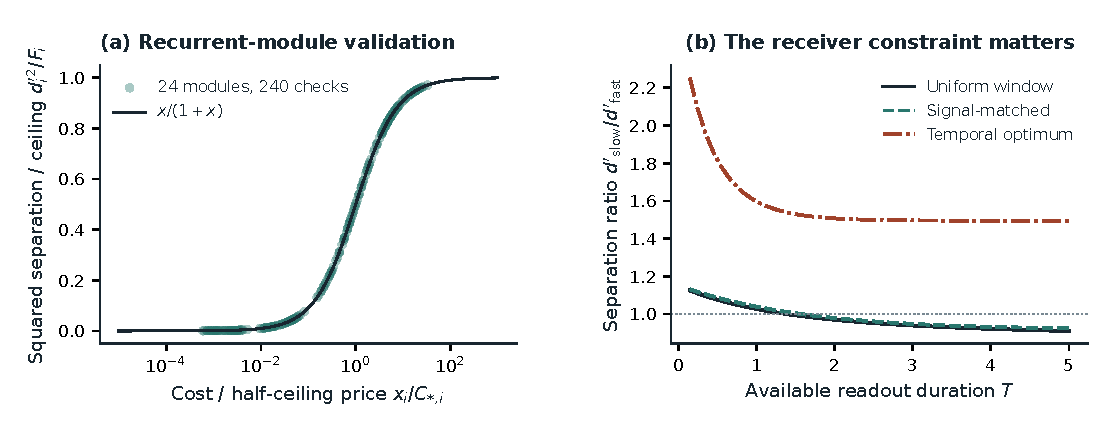
\includegraphics[width=\textwidth]{figures/fig_prrS_allocation_checks.pdf}
 \caption{\textbf{Generality checks and an unconstrained-reader benchmark.}
 (a) The 240 full state-space calculations for 24 recurrent
 module pairs collapse onto the normalized readout-cost law.
 The solid line is \(x/(1+x)\), not a fitted curve.
 (b) Ratios for the original two-pair example with uniform,
 signal-matched and covariance-optimal temporal weights. Only
 the last is allowed arbitrary signed weights adapted to the
 sample covariance. A ratio above one favors the slow output.
 Sampling intervals and model time units are specified in the text.}
 \label{fig:allocationchecks}
\end{figure}


\section{Imposed gain on the FlyWire connectome}
\label{sec:fly}

We ask whether increasing gain on neurons along one anatomical
route can favor its transfer over the other gain state. The two
routes have fixed inputs and outputs, and the simulation does not
infer which neurons a fly modulates. The v783 connectivity table
comes from the whole-brain model
~\cite{shiu2024,dorkenwald2024}. We retain all \(138{,}639\) neurons
with table entries and \(15{,}091{,}983\) directed model edges, and
append 616 release neurons as zero-edge entries [Fig.~\ref{fig:fly}(a)].
The feeding route
uses 21 labellar sugar gustatory receptors and the two bilateral MN9
outputs. The antennal grooming route uses 146 Johnston-organ neurons
and the two published DN1/DN2 outputs. The three endpoint roots that
changed after v630 were mapped using stable supervoxels. Unit-normalized
input indicators and fixed output selections define the simulated
transfer.

We sign synapse counts by inferred transmitter and normalize each
nonempty presynaptic column by its absolute outgoing strength to obtain
\(P\) with \(\|P\|_1\le1\), where \(\|\cdot\|_1\) is the maximum
absolute column sum. For each route we score how easily the inputs
reach each node, and how easily that node reaches the outputs.
These scores sum the first eight steps of propagation using
entrywise absolute weights \(|P|\) forward and \(|P|^\top\) backward,
with weight \(0.85^{h-1}\) for step \(h\). Their geometric mean
gives a score for lying between a route's input and output.
Let \(q_f,q_g\) be these scores at one node for feeding and grooming.
The contrast \((q_f-q_g)\sqrt{q_f+q_g}/(q_f+q_g+10^{-20})\)
favors nodes with a large route difference and appreciable total
support. After excluding endpoints, we select the 256 nodes at
each extreme of this ranking. Selection uses anatomy before
evaluating the signed responses.

In state \(s\), the diagonal matrix \(G_s\) doubles gain on its
256 selected nodes and leaves all other gains at one. The update
matrix \(A_s=0.70I+0.14G_sP\) is stable because
\(\|A_s\|_1\le0.98\). Here \(0.70\) is the self-memory coefficient
and \(0.14\) scales propagation through the graph.

For route \(r\) in state \(s\), let \(T_{r,s}\) be the maximum
sum of squared responses of its fixed outputs to a unit cue at
its inputs, over steps 0 through 24. Each route has a preferred
state: the one that boosts its own selected nodes. Divide its
peak transfer in this state by the peak in the other state.
The route-switch score \(S\) is the geometric mean of the two ratios:
\begin{equation}
  S=\sqrt{\frac{T_{\mathrm{feed},\mathrm{feed}}}
                 {T_{\mathrm{feed},\mathrm{groom}}}
           \frac{T_{\mathrm{groom},\mathrm{groom}}}
                 {T_{\mathrm{groom},\mathrm{feed}}}} .
  \label{eq:switch}
\end{equation}
A value above one favors the assigned states on average. The code
adds the smallest positive normal float before taking each ratio.
As global checks, Fig.~\ref{fig:fly}(b) compares the spectral radius
\(\rho(A_s)\) and the variance from unit independent drive through
40 steps, \(C_H=N^{-1}\sum_{k=0}^{H}\|A_s^k\|_F^2\) at \(H=40\).
We estimate \(C_H\) using the same 16 random sign vectors in each
state. The estimates differ by \(0.016\%\); proximity of these two
summaries does not imply identical spectra or stationary variance.

Feeding and grooming peak transfers are \(21.96\) and \(2.98\)
times larger in their assigned states, respectively
[Fig.~\ref{fig:fly}(c)]. To test whether the route assignment
matters, we keep the selected nodes and shuffle their state labels
within strata with the same transmitter sign and similar in/out
degree and weight. The numerical covariates use separate median
splits of degree, normalized incoming strength, and raw outgoing
strength. The observed \(S=8.08\) exceeds the 95th percentile
\(3.10\) of these shuffles, and none of 999 shuffles reaches it
[\(p=(0+1)/(999+1)=0.001\), the test's resolution limit;
Fig.~\ref{fig:fly}(d)]. This is evidence that the anatomy-based
labels matter in the simulation, not that the gain fields occur
in vivo or that the assigned routes are optimal.

\subsection{Comparison with unmodulated gain}
We also compare each intervention to \(A_0=0.70I+0.14P\), without
changing its input, outputs, or graph. With the same 16 trace probes
and steps 0--40, the estimated per-neuron cost increases by \(0.0083\%\)
for the feeding intervention and \(0.0239\%\) for grooming, relative
to \(A_0\). The paired Monte Carlo standard errors are \(0.0006\) and
\(0.0017\) percentage points, respectively. These are changes in a
graph-wide average when only 256 neurons are modulated, not estimates
of local cost or energetic expenditure. The assigned-route peak squared
transfers rise by factors of \(21.97\) and \(2.98\) relative to \(A_0\).

To compare cue discrimination with the model in the main text, we
average the two fixed outputs of each route over steps 1--24 and use
opposite unit cues at step 0. We add independent unit-variance
noise to every coordinate at each step. For route \(r\), \(b_r\)
is the unit input vector and \(D_r\) selects the two outputs.
The mean for the positive cue is
\(\mu=24^{-1}\sum_{k=1}^{24}D_r A_s^k b_r\).
For innovation step \(\ell\), the matrix of coefficients of the
window average is
\(L_\ell=24^{-1}\sum_{k=\max(1,\ell)}^{24}D_r A_s^{k-\ell}\).
The covariance is \(V=\sum_{\ell\le24}L_\ell L_\ell^\top\); the
pre-cue terms account for stationary background activity.
We compute \(d'=2\sqrt{\mu^\top V^{-1}\mu}\) by adjoint propagation.
Extending the pre-cue history from 40 to 120 steps changes any
covariance entry by less than \(6\times10^{-11}\).
Relative to \(A_0\), the assigned-route window signal amplitudes
increase \(4.91\)- and \(1.67\)-fold; the corresponding \(d'\) ratios
are \(4.90\) and \(1.65\). Thus the modest change in output noise in
this model yields little compression of discrimination over the
tested range. This example is not a test of the one-pass ceiling:
the anatomically derived operator is not constrained to that class,
and the innovations and gain fields are imposed, not fitted.

\begin{figure}[!htbp]
  \centering
  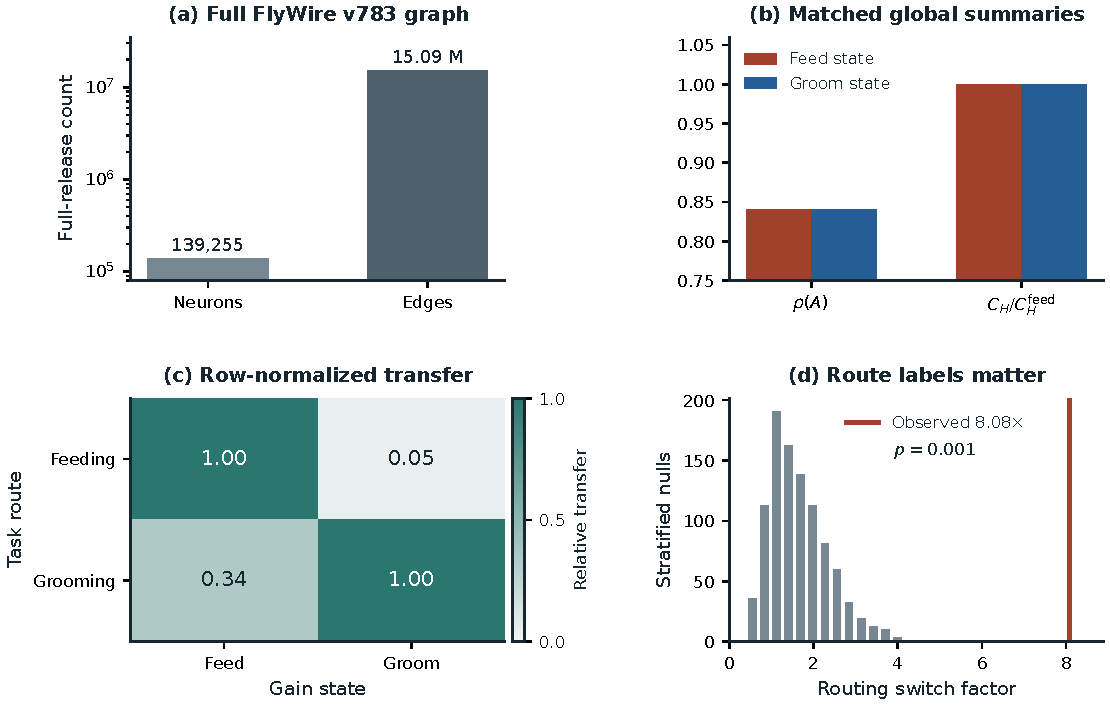
\includegraphics[width=\textwidth]{figures/fig_flywire_gain_routing.pdf}
  \caption{\textbf{Anatomical feasibility in a FlyWire-derived model.}
  (a) Full release scope with all modeled edges and isolated entries.
  (b) Spectral radius and 40-step per-neuron variance, with the latter
  divided by its value in the feeding gain state.
  (c) Peak squared transfer divided by its maximum across the two
  states for each route (each row); the color bar gives relative
  transfer from zero to one. (d) Observed switch score \(S\)
  compared with 999 label shuffles stratified by transmitter sign
  and graph covariates. These are imposed gain states on a fixed
  normalized graph; each state doubles gain on one 256-node module,
  with \(\beta=0.70\) and \(\gamma=0.14\).}
  \label{fig:fly}
\end{figure}

We vary one choice at a time around the default. The first row of
Fig.~\ref{fig:flysens} varies module size \(128,256,512\) (a),
boosted gain \(1.5,2,2.5\) (b), and self-memory
\(\beta=0.60,0.70,0.80\) (c). The second row varies the number of
steps used to select nodes, \(4,8,12\) (d), the damping factor
\(\delta=0.65,0.85,1.0\) (e), and the ranking rule (f). The other
rules rank by \(q_f-q_g\) or by a log ratio of the scores weighted
by \(\sqrt{q_f+q_g}\). When changing the boosted gain \(g_{\rm high}\)
or \(\beta\), we set
\(\gamma=(0.98-\beta)/g_{\rm high}\) in \(A_s=\beta I+\gamma G_s P\)
to retain the common induced-norm stability bound.

Over the 13 unique settings, the switch factors ranged from \(3.51\)
to \(14.98\), and the two-state finite-horizon cost differences remained
below \(0.023\%\). Each score exceeded the 95th percentile of its own
99 newly generated stratified nulls (Fig.~\ref{fig:flysens}). These
are robustness thresholds, not 13 independent significance tests;
the default comparison uses 999 permutations. Varying
the denominator guard in the default ranking from \(10^{-12}\) to
\(10^{-30}\) did not change the selected gain modules. In particular,
these checks do not match the full spectra or prove that the chosen
gain field is optimal or realized in vivo.

\begin{figure}[!htbp]
\centering
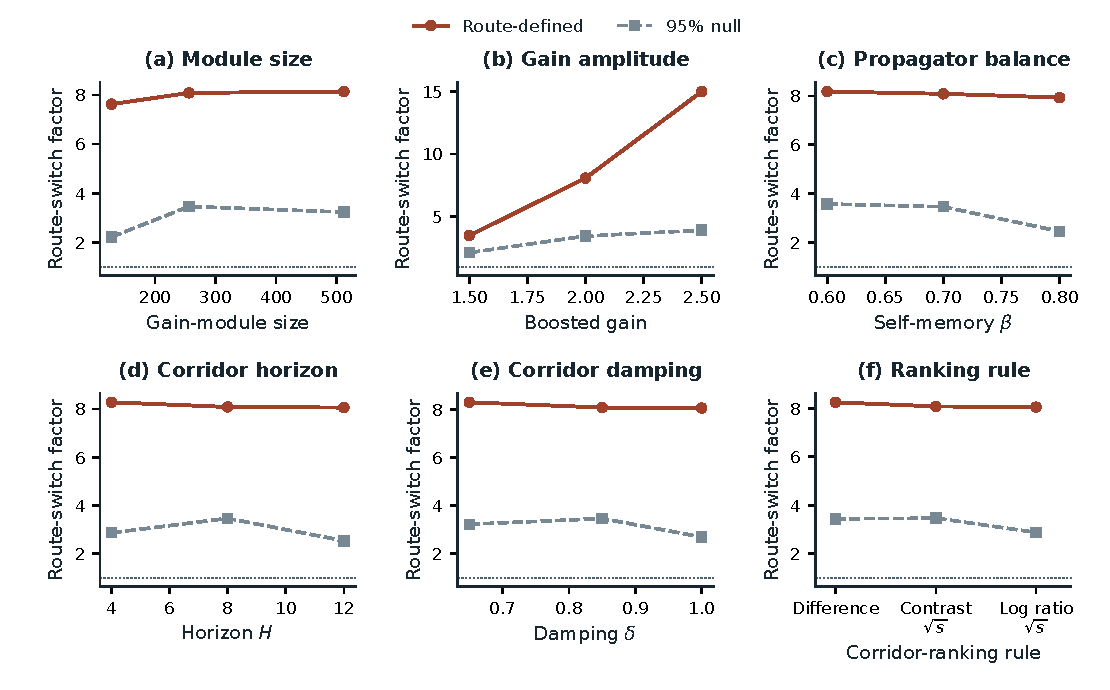
\includegraphics[width=0.97\textwidth]{figures/fig_flywire_gain_routing_sensitivity.pdf}
\caption{\textbf{Sensitivity of the connectome-based example.}
The route-defined switch factor is compared with the 95th percentile
of the stratified nulls for (a) module size, (b) boosted gain,
(c) self-memory at a common stability bound, (d) communicability horizon,
(e) damping and (f) corridor ranking. The default setting is shared
among panels.}
\label{fig:flysens}
\end{figure}

\FloatBarrier
\section{Does a non-normal fit improve prediction in motor cortex?}
\label{sec:alm}

We compare predictions of recovery from photoinhibition in mouse
anterior lateral motor cortex (ALM). The unrestricted and fitted
normal models share eigenvalues and use control trials for fitting.
We then ask whether the unrestricted dynamics better predict late
response magnitude on perturbed trials.

The 18 individually distributed sessions in the bilateral ALM
release~\cite{chen2021modularity,chenli2022dataset} are the starting
cohort, not a selection over the complete archive based on fitted
performance. The excluded session is BAYLORGC85 on 2019-08-03
(fewer than 20 stable high-quality units). The remaining 17 sessions
from six mice enter the analyses at 8, 12 and 16 dimensions.

The analysis retains trials with valid
instruction and timing, no early lick, and units with positive manual
quality scores spanning the selected trials. Sessions require at least
20 such units, at least eight unperturbed trials per instruction, and
at least ten variable units. Spikes are binned at 50 ms and smoothed
with a Gaussian of 50-ms standard deviation. We remove the
control-trial mean time course for each instruction and estimate scales
and principal axes on controls. The one-step full propagator \(A\)
fits residual states in the interval \([-0.85,-0.10)\) s relative to
the go cue, with ridge strength chosen by trial-blocked validation
inside the control set. Identical preprocessing is used for every
comparison.

For the primary normal fit, the rows of \(X\) and \(Y\) are
successive residual states from control trials. We put the full
model's eigenvalues in a real block-normal matrix \(D_N\), using
two-dimensional blocks for complex conjugates. An orthogonal
matrix \(O\) sets the orientation of the normal fit
\(A_N=O D_N O^\top\), without changing those eigenvalues.
We choose \(O\) to minimize mean squared prediction error
\begin{equation}
 L(O)=\frac{1}{nd}\|Y-XA_N^\top\|_F^2,
\end{equation}
where \(n\) counts transitions, \(d\) counts retained principal
components, and \(\|\cdot\|_F\) is the Frobenius norm. We write
\(O=e^K O_0\), where \(O_0\) is a starting orientation and \(K\)
is a real skew-symmetric matrix. This preserves orthogonality,
normality, and the fitted spectrum throughout optimization.
Each fit uses the real-Schur orientation, the identity, and ten seeded
orthogonal starts. We minimize the loss with limited-memory BFGS and
retain the lowest-loss result. This provides a trained comparator,
not a guarantee of the global optimum. The alternative control-window
fit replaces \(A_N\) by \(A_N^5\) in the prediction loss and uses
control early and late averages, with the primary fitted orientation
as an additional start. Both comparisons lock their operators before
evaluating stimulated trials.

For stimulated trials, the input is the observed early average in the
window from \(-0.90\) to \(-0.75\) s; the target is the late average
from \(-0.65\) to \(-0.45\) s. Five discrete propagation steps approximate the
interval between window centers on the 50-ms grid. Evaluation does not
fit dynamical parameters on stimulated trials. For each window's
mean state \(z\), the score uses \(\log(\|z\|_2^2+10^{-9})\),
which we call log-energy. We first regress the predicted and
observed late log-energies separately on the observed early
log-energy. We then compute Spearman correlation between the
two sets of residuals to ask what the dynamics predict beyond
early response size. A sensitivity check also removes inhibition
type and instruction effects. These regressions define the
score; they do not fit the response maps. We average session
scores within each mouse and compare paired differences across mice.

Eigenvalue discrepancies are below \(10^{-14}\), and Frobenius
normality residuals are below \(2\times10^{-15}\) across the saved fits.
At 12 dimensions all selected fits terminated normally. At 16 dimensions
one selected fit per objective reached the iteration cap; the largest
gradient component was below \(7\times10^{-7}\) for both. An
independent finite-difference check uses a real normal operator with
a complex-conjugate pair. Numerical convergence of a local solution
does not establish global optimality.

Table~\ref{tab:alm} shows the primary energy correlation for each
12-dimensional session. The mouse, not the session or stimulated
trial, is the inferential unit. Each mouse's score is the mean over
its included sessions before comparison. The median paired advantage
of the full operator over the one-step-trained normal operator is
\(-0.0129\); three of six paired differences are positive. The
control-window fit gives \(0.0013\), also with three positive
differences [Fig.~\ref{fig:alm}]. Thus an advantage over random
orientations does not establish an advantage over fitted normal
models. This small sample does not establish equivalence either.
In a separate exploratory comparison, we form a second-moment
matrix from mean early responses in each photoinhibition condition.
We compare its principal direction, with and without normalization
by the control activity covariance, to the leading input singular
vector of the five-step map. Covariance weighting improves
absolute cosine alignment in three of six mice (one-sided paired
Wilcoxon \(p=0.656\)). The estimated activity covariance is not the
incoming drive \(Q\) of the theory; neither comparison tests budget
allocation.

\begin{table}[ht]
\caption{\label{tab:alm}ALM held-out energy correlations at 12 dimensions.
Random normal denotes the median over 200 exact same-spectrum controls.
Both trained normal fits use only control trials. Values rounded to
three decimals can conceal small differences; paired inference uses
unrounded session scores.}
\begin{ruledtabular}
\begin{tabular}{llrrrrr}
Mouse & Session & Test trials & Random normal & One-step normal &
Window normal & Full\\
\hline
BAYLORGC85 & 2019-08-02 & 181 & 0.016 & -0.036 & -0.085 & -0.050\\
BAYLORGC85 & 2019-08-05 & 178 & -0.010 & 0.187 & 0.130 & 0.109\\
BAYLORGC85 & 2019-08-08 & 189 & 0.004 & 0.301 & 0.216 & 0.301\\
BAYLORGC88 & 2019-08-26 & 167 & -0.003 & 0.068 & 0.169 & 0.131\\
BAYLORGC88 & 2019-08-27 & 183 & 0.007 & 0.090 & 0.154 & 0.131\\
BAYLORGC89 & 2019-09-26 & 182 & -0.003 & 0.103 & 0.170 & 0.123\\
BAYLORGC89 & 2019-09-27 & 151 & 0.011 & 0.103 & 0.191 & 0.033\\
BAYLORGC89 & 2019-09-30 & 204 & -0.007 & 0.102 & 0.110 & 0.041\\
BAYLORGC90 & 2019-11-18 & 267 & -0.010 & -0.013 & -0.186 & -0.082\\
BAYLORGC90 & 2019-11-20 & 253 & 0.007 & 0.098 & -0.068 & -0.032\\
BAYLORGC90 & 2019-11-21 & 192 & -0.004 & 0.203 & 0.177 & 0.311\\
BAYLORGC94 & 2019-12-04 & 126 & 0.016 & 0.170 & 0.130 & 0.171\\
BAYLORGC94 & 2019-12-05 & 87 & -0.004 & 0.190 & 0.252 & 0.177\\
BAYLORGC94 & 2019-12-06 & 126 & -0.006 & -0.018 & 0.171 & 0.007\\
BAYLORGC95 & 2019-12-13 & 82 & 0.009 & 0.179 & 0.233 & 0.206\\
BAYLORGC95 & 2019-12-16 & 67 & 0.004 & -0.094 & -0.142 & 0.038\\
BAYLORGC95 & 2019-12-19 & 66 & 0.004 & 0.048 & 0.195 & 0.160\\
\end{tabular}
\end{ruledtabular}
\end{table}

\begin{figure}[!htbp]
  \centering
  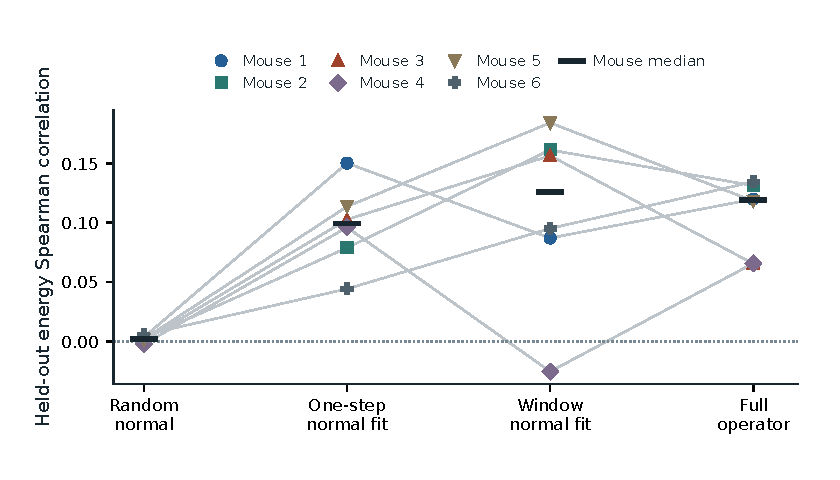
\includegraphics[width=0.76\textwidth]{figures/fig_alm_normal_comparison.pdf}
  \caption{\textbf{Fitting the normal orientation changes the ALM comparison.}
  The held-out Spearman score relates predicted and observed late
  log-response energies after removing dependence on early log-energy.
  Marker shape and color identify mice, averaged across their sessions;
  gray lines connect the same mouse. Dark bars mark across-mouse medians.
  Mouse numbers follow the alphabetical order of animal IDs in Table~\ref{tab:alm}.
  Random normal uses each session's
  median of 200 same-spectrum controls. The two fitted normal models
  preserve the same spectrum but use control trials to choose their
  orientations. The unrestricted full model is fitted on the same
  one-step data as the primary normal fit.}
  \label{fig:alm}
\end{figure}

\FloatBarrier
\noindent\begin{minipage}{\textwidth}
Table~\ref{tab:alm_summary} summarizes both comparators at all three latent
dimensions. No session is excluded based on the fitted spectral radius.
At 8, 12 and 16 dimensions respectively, 15, 16 and 16 of the 17 fits
have spectral radius below one. The few remaining fits are retained for
finite-window prediction and do not serve as examples of the stable
theory. At 12 dimensions, nine of the 16 stable full fits have
\(\max_{0\le k\le20}\|A^k\|_2^2>1\) in the fitted latent coordinates.
This is a diagnostic of the fitted operator, not a measurement of
perturbation gain or evidence that non-normality improves the
recovery-energy endpoint.
\end{minipage}

\begin{table}[!ht]
\caption{\label{tab:alm_summary}Mouse-level ALM differences. Each cell reports
the median paired difference followed by the number of mice favoring the
full operator out of six. For \(r\), positive is higher correlation for
the full operator; for MSE, positive is lower error for the full operator.
MSE differences are in squared latent activity units.}
\begin{ruledtabular}
\begin{tabular}{clccc}
Dimension & Normal orientation fit & Energy \(r\) & Conditioned \(r\) & State MSE\\
\hline
8 & One-step & \(0.0054\) (3) & \(0.0029\) (3) & \(-0.0109\) (2)\\
8 & Window & \(-0.0110\) (2) & \(0.0064\) (4) & \(0.0081\) (4)\\
12 & One-step & \(-0.0129\) (3) & \(0.0033\) (3) & \(-0.0156\) (2)\\
12 & Window & \(0.0013\) (3) & \(0.0103\) (4) & \(0.0047\) (3)\\
16 & One-step & \(-0.0029\) (2) & \(0.0036\) (4) & \(-0.0238\) (2)\\
16 & Window & \(0.0017\) (4) & \(-0.0223\) (1) & \(0.0002\) (3)\\
\end{tabular}
\end{ruledtabular}
\end{table}

\section{Do separate maps for running and stationary trials improve prediction?}
\label{sec:allen}

We compare predictions for the same recorded population during
running and stationary trials, without a targeted perturbation.
We use the Visual Coding Neuropixels session release
~\cite{siegle2021visual}. The 58 session files correspond to 58 distinct
mice. The initial gate requires usable drifting-grating trials, at least
20 trials per state overall, at least five per state within retained
stimulus conditions, and at least 40 qualified units spanning at least
two visual areas. Unit quality filters use presence ratio
\(\ge0.95\), amplitude cutoff \(\le0.1\), interspike-interval
violations \(\le0.5\), and the good-quality label when available.
Running is defined by mean wheel speed greater than \(1\,\mathrm{cm/s}\)
in the stimulus window. Units are held fixed across the states within
a session. Twenty-two mice pass the initial gate.

In the stricter analysis, we match running and stationary trials by
nearest time within the same orientation and temporal frequency and
within 300-s acquisition blocks. Retained conditions must support at
least three pairs, and mice must provide at least 20 pairs across two
or more conditions. Fourteen mice provide 869 pairs and 3954 units.
The example in Fig.~\ref{fig:allen}(a) shows firing rates from
the same units in the two conditions.
This expanded analysis was designed after the initial pilot outcomes
were available, and is an exploratory robustness analysis.

Spikes are binned at 20 ms without smoothing; the first 100 ms after
onset are omitted. State- and condition-specific mean time courses are
estimated on training trials and subtracted. Scaling, a shared PCA
basis, and ridge selection use training data only. Pairs stay together
in trial partitions. If \(A_s\) is the fitted one-bin map for
behavioral state \(s\), \(A_s^5\) predicts residual activity
five bins (100 ms) later. The primary comparators are a
common pooled matrix and a nonnegative scalar rescaling of it in
each state. A latent-coordinate diagonal gain is a secondary
statistical comparator, not a model of identified cellular gains.
Prediction improvement \(\Delta R^2\) is the decrease in mean squared
error relative to the comparator, normalized to zero-predictor error
within state and averaged equally over the two states.

Each of the 999 nulls swaps labels within matched pairs and refits
all preprocessing and models, keeping held-out pair assignments fixed.
The group comparison uses mouse medians; the raw \(p=0.001\) for both
primary controls is the resolution limit, and Holm correction gives
\(p=0.002\). This is a local exchangeability approximation: it does
not eliminate unmeasured state variables or fully preserve long
behavioral episodes. Figure~\ref{fig:allen}(b) compares the prediction
improvement against all three comparators.
At 12 dimensions the median gain over the scalar comparator is
\(0.00601\), compared with \(0.00677\) and \(0.00467\) at 8 and
16 dimensions. The advantage is smaller over the latent diagonal-gain
comparator: median \(0.00505\), positive in 12 of 14 mice. That
comparator is in fitted latent coordinates and does not implement
the anatomical gain field of the two-output construction. The
temporal-block and population-mean-removal
sensitivities give \(0.00563\) and \(0.00912\), respectively
[Fig.~\ref{fig:allen}(d)].

To compare maps apart from scalar gain, we divide each \(A_s^5\)
by its Frobenius norm and measure the Frobenius norm of their
difference. Its median is \(1.085\), with \(p=0.001\) against
refitted group nulls [Fig.~\ref{fig:allen}(c)]. The distance includes
changes of relative channel weights as well as possible rotation.
Only four mice have sufficient trials to estimate the map differences
in independent halves, with at least two trials per condition and
state in each half and at least five pairs per half. Three of the four
half-split cosines are positive; their median is \(0.330\) with an
animal bootstrap interval \([-0.044,0.480]\). We do not infer
consistent leading-direction rotation from this limited subset.
The 28 main fits are stable but their 100-ms squared gains are all
below one; the fits do not demonstrate amplification at that horizon.

\noindent\begin{minipage}{\textwidth}
Filtered pupil-area traces are available in 17 of the 22 initially
eligible sessions. Requiring at least 80\% pupil coverage and
matching within a 0.5-session-SD pupil caliper, in addition to stimulus
and time matching, leaves no mouse with adequate pair support.
An exploratory training-only additive linear and quadratic adjustment
retains eight mice. In the same pupil-valid trials, the median
advantage over scalar gain is \(0.00434\) without adjustment and
\(0.00480\) with adjustment, with six positive mice in both cases.
The corresponding 95\% mouse bootstrap intervals are
\([-0.00548,0.01239]\) and \([-0.00223,0.00954]\).
This analysis is inconclusive about a locomotion-specific effect
independent of arousal; neither estimate supports dismissing that
alternative. Spectra and costs are not matched between the recorded
states, and the predicted residual is not an externally perturbed
input--output response.
\end{minipage}

\begin{figure}[!htbp]
\centering
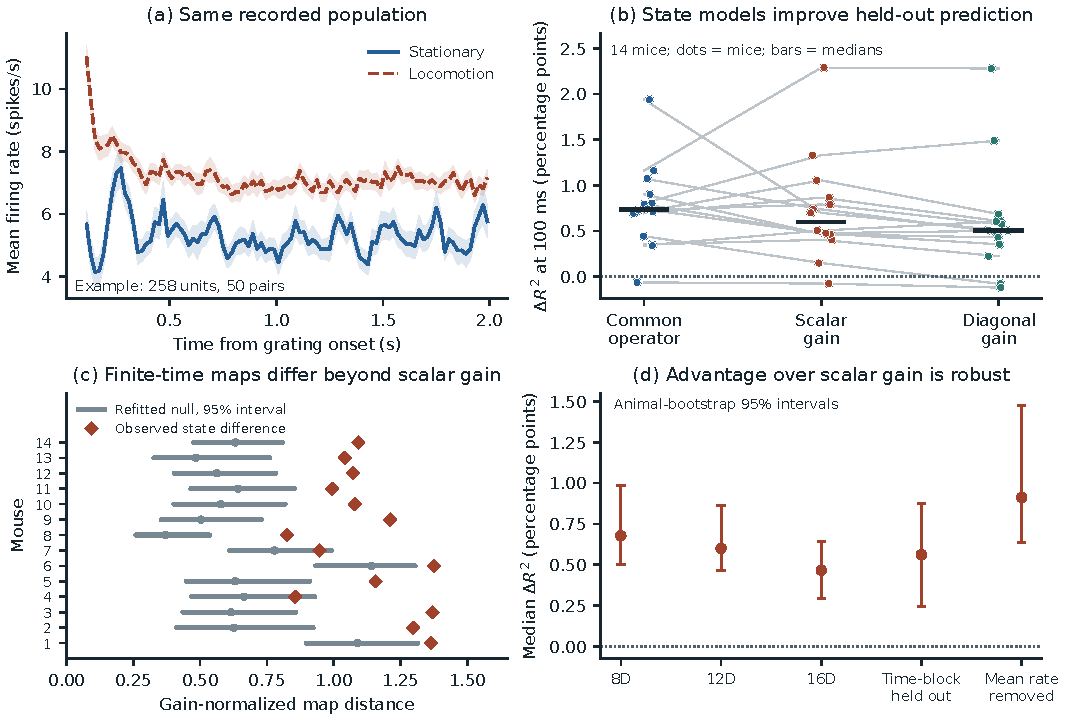
\includegraphics[width=\textwidth]{figures/fig_allen_state_routing.pdf}
\caption{\textbf{State-associated effective response maps in the same
recorded populations.} (a) Example of matched stimulus trials from
258 units; shading is trial standard error. (b) Held-out 100-ms
prediction improvements over three comparators, in percentage
points. Dots denote mice, connected across comparators; bars mark
medians. (c) Diamonds show each mouse's difference between
gain-normalized maps; gray intervals show the central \(95\%\) of
999 within-pair shuffles with refitted maps. (d) Improvement over
scalar gain across dimensions, held-out time blocks, and subtraction
of population mean activity; intervals resample mice. These comparisons do not identify
causal transfer or matched-cost optimization.}
\label{fig:allen}
\end{figure}

\FloatBarrier
\clearpage
\section{Predictive allocation tests and the reversal region}
\label{sec:predictivetests}

\subsection{Fixed protocol for heterogeneous recurrent pathways}

To distinguish prediction from a fitted response curve, we generate
a new fixed set of eight synthetic networks using seed 20261110.
Their pathway counts are \(2,4,6,8,2,4,6,8\), giving 40 pathways.
Each source and output population has two to four coordinates.
Dense off-diagonal entries have magnitude \(0.02\)--\(0.20\);
the diagonal leak exceeds each absolute row sum by an independent
margin in \(0.35\)--\(1.1\). Each internal matrix is then scaled
by a factor in \(0.5\)--\(1.6\). Alternating network cases have
positive or signed off-diagonal entries. Thus stability is fixed
by construction, and both populations contain recurrent cycles.
The forward matrix is positive and Frobenius-normalized.
Independent diagonal source and output drive intensities are in
\(0.35\)--\(1.7\). Cue and scalar readout vectors are uniform
unit vectors on their respective populations. These choices were
fixed before this run; networks are not selected for an allocation
effect or a ranking reversal.

At unit forward gain, 48-node Gauss--Legendre quadrature determines
the readout mean \(h_i\) and the separate local and propagated
variances \(L_i,S_i\) for windows \(T=0.35,1.6\). A stationary
source-drive calculation gives \(\kappa_i\). The derived
\(F_i=4h_i^2/S_i\) and \(C_{*,i}=\kappa_iL_i/S_i\) then predict
allocations without fitting a gain--discrimination curve.
Each network uses three budgets: \(0.25,1,4\) times its total
unit-gain excess cost \(\sum_i\kappa_i\). The same three budgets
are held fixed across the two windows, giving 48 settings.

For an independent numerical comparison, the optimization objective
uses the full generator at each candidate gain. A Lyapunov solve
computes its stationary covariance, and matrix-exponential integral
identities compute its cue mean and window variance. It does not
evaluate the rational cost law in the objective. Budget shares
\(z_i\) parameterize gains as
\(m_i=\sqrt{Bz_i/\kappa_i}\), with \(z_i\ge0\) and
\(\sum_i z_i=1\). The resulting full-state stationary cost is
also checked directly. Joint discrimination is optimized by SLSQP
from three fixed types of starts: uniform, seeded Dirichlet, and
the first-coordinate corner. All 144 joint starts converge; their
statuses and objectives are retained. Max--min discrimination is
checked by a separate epigraph optimization of the full-state
scores. The analytical unequal-ceiling max--min prediction uses
the scalar target equation derived in Sec.~\ref{sec:modularsupp}.

The maximum relative objective discrepancies are
\(2.5\times10^{-13}\) for joint and \(2.4\times10^{-11}\) for
max--min decoding. The largest joint budget-share discrepancy is
\(7.1\times10^{-7}\), and the largest relative total-cost error
is \(1.9\times10^{-14}\). Main Fig.~4(e,f) shows joint predictions
and gains over equal shares; Fig.~\ref{fig:strengthening}(c) gives
the independently optimized max--min comparison. These checks
validate the allocation predictions on full recurrent models;
they do not infer a biological distribution of optimal policies.

For joint utility \(U=d_{\rm joint}'^2\), the relative improvement
\(100(U^*-U_{\rm equal})/U_{\rm equal}\) ranges from
\(0.0067\%\) to \(44.6\%\), with median \(3.31\%\).
The medians at the two windows are \(7.40\%\) and \(2.95\%\).
The unit-gain matrices, drives, cues and all three budgets are
unchanged across windows. The median total variation of the
optimal joint shares between windows is \(0.101\), with total
variation defined as half the sum of absolute share changes
[Fig.~\ref{fig:strengthening}(d)]. Settings with nearly equal
prices and returns can have almost no benefit from reallocation;
the optimization does not imply that equal allocation is always
substantially inefficient.

\subsection{Fixed-cost region and explicit noise interventions}

Main Fig.~3(e) scans 141 rate ratios \(R\in[1.05,8]\) and
161 coupling ratios \(\gamma\in[1.01,8]\), giving 22,701
specified model points. Set \(a_s=R^{-1/2}\), \(a_f=R^{1/2}\),
so \(a_sa_f=1\). For each point choose
\[
 \kappa=[2a_sa_f(a_s+a_f)]^{-1},\qquad
 m_f^2=\frac{1.25712}{\kappa(1+\gamma^2)},\qquad m_s=\gamma m_f.
\]
Thus the entire grid has the same excess cost, not the same
absolute gains. The exact eventual-reversal interval is
\(\sqrt R<\gamma<R\). Requiring opposite rankings at both
\(T=0.5\) and \(T=3\) selects the narrower region
\[
 \frac{V_0(a_s,0.5)}{V_0(a_f,0.5)}<\gamma^2<
 \frac{V_0(a_s,3)}{V_0(a_f,3)}.
\]
All grid classifications agree with this interval; 3,057 grid
points pass the two-window test. The color encodes the smaller
of the two fractional winning margins, in percent. The largest
such minimum margin in this grid is \(11.1\%\). These counts
describe a chosen parameter grid, not a prevalence estimate or
a statistical significance calculation. A prescribed coarse subset
of 32 two-route settings, spanning four rate ratios, four coupling
ratios and two windows, is also checked by full-state Lyapunov
and matrix-exponential calculations rather than the scalar ratio.

The explicit noise interventions in main Fig.~3(c) hold the
couplings fixed. Removing local output drive ties the two
separations. Removing source drive changes their ratio but not
its crossing. These are mechanism controls, not matched-cost
comparisons between different drive covariances. Return-coupling,
colored-drive and temporal-weight sensitivity examples are preserved
in Fig.~\ref{fig:strengthening}(a), with their full grid and
unsuccessful cases reported in Sec.~\ref{sec:crosssupp}.

\subsection{A condition-violating control}

The local-noise endpoint test requires common signal and
propagated-noise terms and a common price coefficient. To expose
the consequence of violating these assumptions, multiply only
the slow route's source-drive intensity by four, keeping its
local output drive unchanged. Set the gains to \(1.17,0.90\),
so its excess-cost coefficient is four times larger and the
actual budget ratio remains \(6.76\) at total excess cost
\(1.25712\). The local-noise endpoint ratios remain four and
16. Nonetheless, no separation-rank crossing occurs on the tested
\(0.025\le T\le12\) range [Fig.~\ref{fig:strengthening}(b)].
Using the endpoint inequality without checking matching would
therefore be incorrect. This is not a failure of the individual
module law: the unequal \(F_i\) and \(C_{*,i}\) still give the
correct scores. The heterogeneous recurrent allocation tests
above deliberately allow unequal coefficients and do not assume
that their pathways satisfy the controlled reversal criterion.

\begin{figure}[!htbp]
\centering
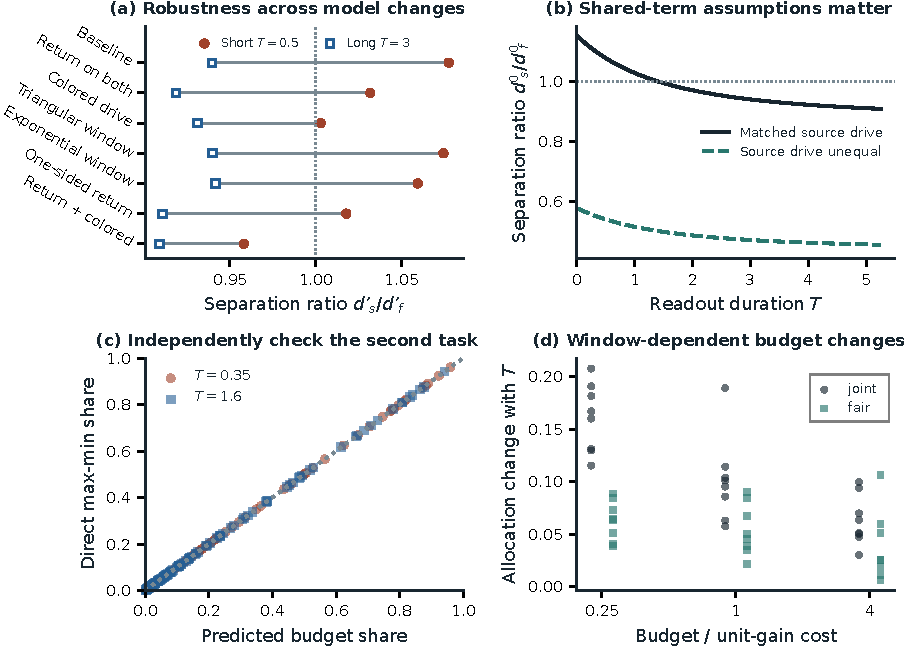
\includegraphics[width=\textwidth]{figures/fig_prrS_strengthening.pdf}
\caption{\textbf{Sensitivity, matching conditions and recurrent allocation.}
(a) Sensitivity examples with horizontal labels:
rust circles are \(T=0.5\), blue open squares \(T=3\). Return
coupling has magnitude \(0.05\), and colored-drive time constant
is \(0.5\); the combined case is retained. (b) Baseline matched
drive (dark solid) versus a fourfold source-drive mismatch on the
slow route (teal dashed), both at excess-cost ratio \(6.76\).
The latter does not satisfy the endpoint test's shared-term
assumptions. (c) Predicted versus full-state max--min budget shares
for the 48 heterogeneous recurrent settings. Colors and symbols
identify the two windows as in main Fig.~4(e); dotted line is
equality. (d) Total-variation changes in optimal budget shares
between \(T=0.35\) and \(1.6\), at each unchanged total budget.
Dark circles denote joint decoding and teal squares max--min;
each group contains eight fixed network examples. No biological
sampling or significance inference is intended.}
\label{fig:strengthening}
\end{figure}

\FloatBarrier
\section{Finding a max--min allocation from decision feedback}
\label{sec:feedbacksupp}

\subsection{Budget conservation and convergence}

For a fixed readout window, let
\(f_i(x_i)=F_i x_i/(x_i+C_{*,i})\) be squared cue discrimination
with positive \(F_i,C_{*,i}\), as derived in
Sec.~\ref{sec:modularsupp}. For equiprobable cues with Gaussian
readout distributions of opposite means and equal variance,
the zero-threshold decision has correctness probability
\(\pi_i(x_i)=\Phi(\sqrt{f_i(x_i)}/2)\), where \(\Phi\) is the
standard normal cumulative distribution function. This transform
is the same and strictly increasing for all outputs, so maximizing
the worst correctness probability also maximizes the worst \(d'\).
The rule takes budget from outputs above mean correctness and gives
it to outputs below the mean:
\(\dot x_i=\eta(\bar\pi-\pi_i)\), where
\(\bar\pi=n^{-1}\sum_i\pi_i\), \(\eta>0\), and \(n\) is the number
of separately required outputs. The sum of the updates is zero.
If \(x_i=0\), then \(\pi_i=1/2\), while at least one other output
has positive budget and \(\pi_j>1/2\); the vector field therefore
points into the feasible set.

On the simplex \(\sum_i x_i=B>0\), define
\begin{equation}
 V(\boldsymbol{x})=\sum_i\int_0^{x_i}\pi_i(u)\,\dd u,
 \qquad
 \dot V=-\eta\sum_i(\pi_i-\bar\pi)^2 .
 \label{eq:feedback_lyap}
\end{equation}
The field is continuous, and solutions from the same point are
unique: the derivative of half the squared distance between any
two solutions \(\boldsymbol{x},\boldsymbol{y}\) on the simplex
is \(-\eta\sum_i(x_i-y_i)[\pi_i(x_i)-\pi_i(y_i)]\le0\).
The simplex is compact, and the only invariant set with
\(\dot V=0\) is the unique equal-correctness point. To see uniqueness
and optimality, the minimum budget for a common target probability
\(\pi>1/2\) is \(\sum_i\pi_i^{-1}(\pi)\), which is strictly increasing
up to the smallest ceiling, where it diverges. The largest feasible
target exhausts \(B\), and no allocation can exceed it. Thus
the continuous mean-feedback rule converges globally to the max--min
allocation. It is not a solution to the joint-decoding objective.

\subsection{Finite batches and a change of readout window}

We use the two independent pairs of
Sec.~\ref{sec:crosssupp}, with \(B=1.25712\) and \(\kappa=0.2\).
The environment converts budgets to gains through
\(m_i=\sqrt{x_i/\kappa}\). For each fixed gain during a batch,
stationary Lyapunov and matrix-exponential calculations give the
Gaussian readout moments. Trials begin from the stationary
background at that gain before the cue is applied. With balanced
cue probabilities and a fixed zero-threshold decision, a count
of correct decisions in 32 independent trials per output is drawn
directly from the equivalent binomial law. The controller sees
only these counts. It uses neither the moments nor the target
allocation. If \(k\) is the batch index, the slow budget is updated
by adding \(\eta_k(\widehat\pi_{\rm f}-\widehat\pi_{\rm s})\)
and clipping to \([0,B]\); the fast budget is its complement.
Here \(\widehat\pi_i\) is the fraction correct in the batch and
\(\eta_k=0.20B/[1+(k-1)/50]^{0.65}\). The reported shares average
the second half of each run. In the chance-feedback control,
independent fair binary outcomes replace correctness, with the
same random draws for the two windows.

We use 512 replicates per condition and start the slow budget
at \(0\), \(1.09512\), or \(B\). The matched-pair optima at
\(T=0.5\) and \(3\) assign it \(0.834\) and \(0.902\) of the
budget, respectively. Starting at the figure's fixed allocation,
the update moves in the predicted direction in \(99.0\%\) and
\(99.8\%\) of runs after 4,096 batches, versus \(64.6\%\) and
\(62.1\%\) after 64 batches. From the other two starts, the final
median shares are \(0.831\)--\(0.832\) for the short window and
\(0.900\)--\(0.901\) for the long window. When switching from
the learned short-window allocation to the long window, we
restart the step-size schedule at the announced block change.
All replicates increase the slow share. The chance-feedback
control cannot distinguish the windows and is much more variable.

\begin{table}[!htbp]
\caption{\label{tab:feedback}Simulated feedback on the two-pair
example. Entries are the median slow-route budget share after
4,096 batches, with 10th--90th percentiles across 512 replicates.
The fixed initial share for the two single-window runs is \(0.871\).}
\begin{ruledtabular}
\begin{tabular}{lcc}
Feedback and window & Exact target & Learned share \\
\hline
Correctness, \(T=0.5\) & 0.834 & 0.830 [0.803, 0.852] \\
Correctness, \(T=3\) & 0.902 & 0.900 [0.889, 0.911] \\
Correctness, switch \(0.5\to3\) & 0.902 & 0.901 [0.889, 0.910] \\
Chance, either window & --- & 0.792 [0.473, 0.958] \\
\end{tabular}
\end{ruledtabular}
\end{table}

The final run uses 131,072 decisions per output and window.
For the fixed start, median gains in worst-output correctness
are \(0.43\) and \(0.06\) percentage points, respectively;
some long-window runs worsen performance. The result establishes
feasibility with task feedback, not trial efficiency.

\subsection{Four heterogeneous recurrent pathways}

We use the first four-pathway network (case 1, zero-based) from
Sec.~\ref{sec:predictivetests}, at both original windows
\(T=0.35,1.6\) and the original unit-gain total budget
\(B=\sum_i\kappa_i\). The within-module recurrent dynamics,
cue and readouts are unchanged. We keep the two-pair protocol's
batch size, step-size schedule, and number of batches and replicates.
We use equal shares and all four simplex vertices as initial
allocations. For each batch, the controller adds
\(\eta_k(\overline{\widehat\pi}-\widehat\pi_i)\) to each
allocation and projects the resulting vector onto the nonnegative
simplex of total budget \(B\). This is the same budget-space
update as clipping one share and taking its complement in the
two-pathway case. The finite-batch correctness counts are drawn
from the Gaussian readouts as above, using full-state moments
checked at multiple gains. The analytic max--min allocations are
used only for evaluation, not for the updates.

Figure~\ref{fig:feedbacksupp} shows the tradeoff between feedback
volume and performance. From equal shares, at 2,048 decisions per
output the median total-variation errors in the budget shares are
\(0.158\) and \(0.077\) at the short and long windows. Nonetheless,
the median gains in worst-output correctness are already \(0.55\)
and \(1.39\) percentage points, compared with the attainable
\(0.90\) and \(1.82\). At 131,072 decisions, the median errors
fall to \(0.024\) and \(0.012\) and the gains rise to \(0.78\)
and \(1.71\) points. From the four vertex starts, final median
errors range from \(0.024\) to \(0.033\) at the short window
and \(0.011\) to \(0.012\) at the long window. Chance feedback
from equal shares leaves final median errors of \(0.467\) and
\(0.446\) and reduces median correctness at both windows.
Thus useful improvements do not require pinpointing the optimal
allocation in this example. The achievable gains are larger than
for the starting allocation used in the two-pathway example.
These are two windows of one recurrent model, not independent
network or animal samples.

\begin{figure}[!htbp]
\centering
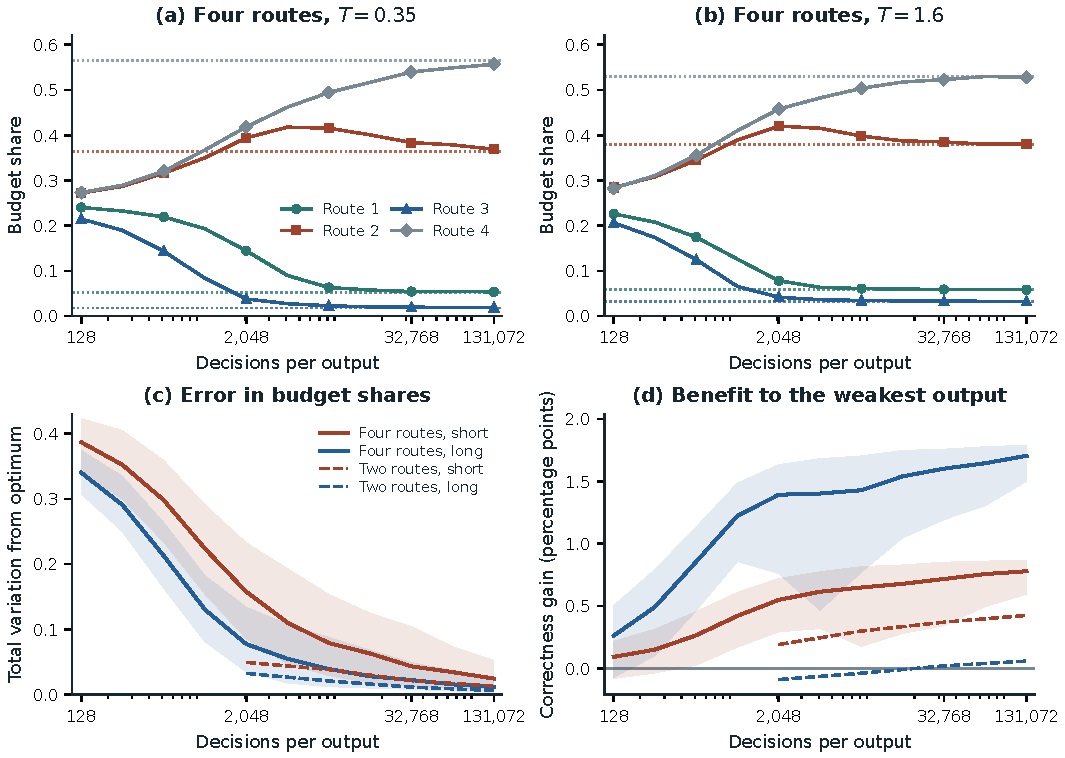
\includegraphics[width=\textwidth]{figures/fig_prrS_feedback.pdf}
\caption{\textbf{Finite decision feedback improves the weakest output
before the budget shares fully settle.}
(a,b) Median shares across 512 runs of the four-pathway model,
initialized at equal shares. Color and marker identify each route;
horizontal dotted lines give its analytic max--min share.
(c) Allocation error, defined as half the sum of absolute share
differences from the optimum. (d) Gain in worst-output correctness
relative to the initial allocation, in percentage points. Solid
curves show four-route medians; shaded bands give the 10th--90th
percentiles across runs. Dashed curves show two-route medians from
the fixed allocation in Table~\ref{tab:feedback}. Short and long
windows are \(0.35,1.6\) for four routes and \(0.5,3\) for two routes.
Each checkpoint scores the allocation averaged over the second
half of that run prefix, not the average correctness during training.}
\label{fig:feedbacksupp}
\end{figure}

\subsection{What the controller implements}

The model assumes labelled or otherwise evaluable decisions, an
externally maintained pool of excess variance, and a calibrated
budget-to-gain map. It evolves \(x_i\), not \(m_i\). Directly
differentiating \(x_i=\kappa_i m_i^2\) would divide by \(m_i\),
which is singular at zero; the budget-space rule is well defined
there and does not furnish a smooth biophysical gain law.
The binomial counts reproduce decision statistics for independent
stationary Gaussian trials at each fixed allocation. They do not
simulate activity transients during gain changes or correlations
between trials. The feedback experiment tests whether an allocator
can use task performance to approach the optimum under these
assumptions, not whether biological circuits implement the allocator.

\FloatBarrier
\section{A local activity-feedback model for coupling gains}
\label{sec:localgainsupp}

\subsection{Pairwise exchange replaces a global comparison}

Let \(b_i\) be a route's target excess variance, with \(b_i\geq0\)
and \(\sum_i b_i=B\). The routes exchange this target budget along
a connected graph with symmetric weights \(w_{ij}\geq0\). When
the realized cost \(x_i=\kappa_i m_i^2\) tracks \(b_i\) exactly,
the rule is
\begin{equation}
  \dot b_i=\eta\sum_j w_{ij}[\pi_j(b_j)-\pi_i(b_i)].
  \label{eq:edgefeedback}
\end{equation}
Here \(\pi_i\) is the expected correctness probability defined in
Sec.~\ref{sec:feedbacksupp} for a fixed readout window. Exchange
on an edge cancels from the total budget. At a zero budget the
correctness probability is at chance, so the field does not point
out of the simplex. With \(V(\boldsymbol b)=\sum_i\int_0^{b_i}
\pi_i(u)\,\dd u\),
\begin{equation}
 \dot V=-\frac{\eta}{2}\sum_{ij} w_{ij}(\pi_i-\pi_j)^2.
\end{equation}
On the fixed-budget plane, uniqueness of trajectories also follows
from contraction in the quadratic distance defined by the Laplacian
pseudoinverse: the derivative of half that distance squared for two
solutions is \(-\eta\sum_i(b_i-\widetilde b_i)
[\pi_i(b_i)-\pi_i(\widetilde b_i)]\leq0\). By connectedness,
zero dissipation requires all outputs to have equal correctness.
On the compact simplex this gives global convergence to the unique
max--min allocation, by the common-target argument in
Sec.~\ref{sec:feedbacksupp}. No node needs the global mean correctness.
The network is given a total target budget through initialization;
it does not learn the value of \(B\).

\subsection{Estimating the cost and adjusting the actual gain}

The source-driven component of the output under a fixed unit
gain satisfies \(\dot r_i=D_i r_i+B_i u_i\).
If the output-local noise is independent of the source noise,
then in stationarity \(v_i=v_i^{\rm local}+m_i r_i\), and
\begin{equation}
 \kappa_i=\Tr\operatorname{Cov}(r_i),\qquad
 \tau_\kappa\dot{\hat\kappa}_i=\|r_i\|^2-\hat\kappa_i,
 \qquad
 \dot m_i=\gamma(b_i-\hat\kappa_i m_i^2).
 \label{eq:gainhomeostasis}
\end{equation}
The variance estimate uses zero-mean cue-free activity. The filter
must represent the source-driven response, not total output activity;
for a recurrent module it requires access to the incoming drive and
a copy of the output filter, potentially with several state variables.
Neither the analytic coefficient \(\kappa_i\) nor the optimal gain
enters the updates. At a positive fixed \(b_i\) and exact cost
estimate, the gain drifts monotonically toward
\(\sqrt{b_i/\kappa_i}\) from either side. At \(m_i=0\) it has finite
derivative \(\gamma b_i\). The actuator changes the forward block
only, so it leaves the frozen neural decay spectrum unchanged.
This does not imply that the covariance during adaptation is
stationary. In particular, \(\sum_i b_i\) is conserved, but the sum
of the frozen-gain costs \(\sum_i\kappa_i m_i^2\) need not be
exactly \(B\) while the gains are adjusting.

For the deterministic mean model, let the edges compare the
stationary readout probabilities \(\pi_i(x_i)\) at the actual gains.
At the interior optimum with
\(\hat\kappa_i=\kappa_i\), the budget and realized costs agree.
Write \(y=\delta\boldsymbol x\), \(z=\delta\boldsymbol b\),
\(H=\operatorname{diag}(\pi_i'(x_i^*))>0\),
\(G=\operatorname{diag}(2\gamma\kappa_i m_i^*)>0\), and let
\(L\) be the symmetric graph Laplacian. The linearized equations
at fixed cost estimates are \(\dot z=-\eta LH y\) and
\(\dot y=G(z-y)\). Eliminating \(z\) yields
\begin{equation}
 HG^{-1}\ddot y+H\dot y+\eta HLHy=0,
 \qquad \mathbf{1}^{\mathsf T}(y+G^{-1}\dot y)=0 .
\end{equation}
The energy \((\dot y^{\mathsf T}HG^{-1}\dot y+
\eta y^{\mathsf T}HLHy)/2\) decreases at rate
\(-\dot y^{\mathsf T}H\dot y\). On the constrained subspace it is
positive definite: its only possible zero has \(\dot y=0\),
\(Hy\) constant, and \(\mathbf{1}^{\mathsf T}y=0\), which forces
\(y=0\). The same argument makes the largest invariant set at
zero dissipation the origin. Thus the interior equilibrium is
locally exponentially stable for finite positive adaptation rates in
this continuous mean model. If the estimate obeys the averaged
filter equation, its deviations decay independently because the
source-driven filter is gain-independent; the linearized system
adds a stable block. This is not a proof of global stability for
the coupled, sampled stochastic model with noisy estimates.

\subsection{Simulation with continuous background activity}

We use the two-pair example and the first four- and eight-pathway
networks from Sec.~\ref{sec:predictivetests} (cases 1 and 3), at their
original windows and budgets. The regulating graph is a unit-weight
open chain, distinct from the fast neural connectivity. The two-pair
run starts at the Fig.~3 gains; the heterogeneous runs start at unit
gains or zero gains with equal target shares. We retain the size
and step schedule of the finite-feedback batches in
Sec.~\ref{sec:feedbacksupp}, using 48 replicates per condition.
In each batch we compare neighboring estimates of correctness and
apply antisymmetric transfers. If total outgoing flow would exceed
a donor's target budget, all outgoing flows from that donor are
scaled by the same factor. This prevents negative budgets without
a centralized projection or a violation of budget conservation.

We propagate the source, output-local component and unit-gain filter
through each readout window and an intervening cue-free gap of one
model time unit by exact Gaussian transitions. The readout integrals
are included in the transitions. Between batches the gain is updated
by integrating Eq.~\eqref{eq:gainhomeostasis} over one unit of slow
controller time, holding its target and estimate fixed during that
update. Within a batch the gain is fixed. The residual source-driven
output \(v_i-v_i^{\rm local}-m_i r_i\) carries forward across gain
changes and decays with \(D_i\); the stochastic activity is not reset.
To isolate responses to brief test cues, each labelled probe adds the
linear cue response for its own readout window, without carrying its
deterministic tail to the next probe. This leaves the continuous
background trajectory unchanged. The squared norm of the filter at
the end of each blank provides the cost sample; 4,096 cue-free samples
initialize the estimate (discarding the first quarter). Subsequent
batch means update it with an exponential time constant of 256
batches. The nominal gain actuator rate is \(\gamma=0.5\);
a separate short-window four-route test slows it by a factor of 64.

For binary feedback the controller uses fraction correct. The
alternative uses the mean divided by the sample standard deviation of
the cue-aligned scalar readout, passed through the standard Gaussian
CDF. In the stationary large-sample limit both signals estimate the
same correctness; the latter uses more information from each labelled
trial and can be biased at finite batch size. Neither uses the analytic
cost coefficients. For evaluation only we use those coefficients to
measure the frozen-gain cost and allocation. We average those costs
over the second half of each run prefix; we also retain instantaneous
cost errors. Correctness computed from averaged costs is an evaluation
at frozen gain, not the observed trial accuracy during training.

\subsection{What the feedback loop reaches with finite data}

For the two-pair model, the final median gain-implied slow-route
cost divided by \(B\) is \(0.826\) at the short window and
\(0.898\) after switching to the long window (targets: \(0.834\)
and \(0.902\)). The controller restarts the step-size schedule at
the announced switch but carries its budgets, gains, cost estimates
and background states across it [Fig.~\ref{fig:localgainloop}(a)].

In the four-route model the final median total-variation errors are
\(0.025\) and \(0.009\) with margin feedback, or \(0.024\) and
\(0.014\) with binary feedback. Zero-gain starts reach similar
errors under margin feedback. The eight-route model also approaches
the target at the long window (median error \(0.024\) with margin
feedback), but remains farther from optimal at the short window
(\(0.152\)), despite nearly matching total cost. All runs use the
same 131,072 labelled decisions per output, in addition to cue-free
calibration activity. These results show that regulating total cost
is not sufficient to allocate it well.

Under nominal actuation, the four- and eight-route margin runs
end with median absolute total cost errors of \(0.28\%\) to
\(0.47\%\) for the averaged allocations. The instantaneous errors
at the final checkpoint have medians from \(0.55\%\) to \(1.01\%\).
Slowing the gain actuator in the four-route short-window run raises
the averaged cost error to \(6.25\%\) at 16,384 decisions, versus
\(0.66\%\) at the nominal rate, although it declines later.

Margin feedback is not uniformly more efficient than binary
feedback at the same number of labelled decisions. In the short-window
four-route example the median frozen-gain correctness gain at 2,048
decisions is \(0.15\) percentage points with margins versus \(0.13\)
with binary feedback. The eight-route short-window run initially
loses correctness with either signal, and the final median gains
are only \(0.20\) and \(0.19\) points, respectively. The rule is a
candidate for slow adaptation, not evidence for fast routing in vivo.

\begin{figure}[!htbp]
\centering
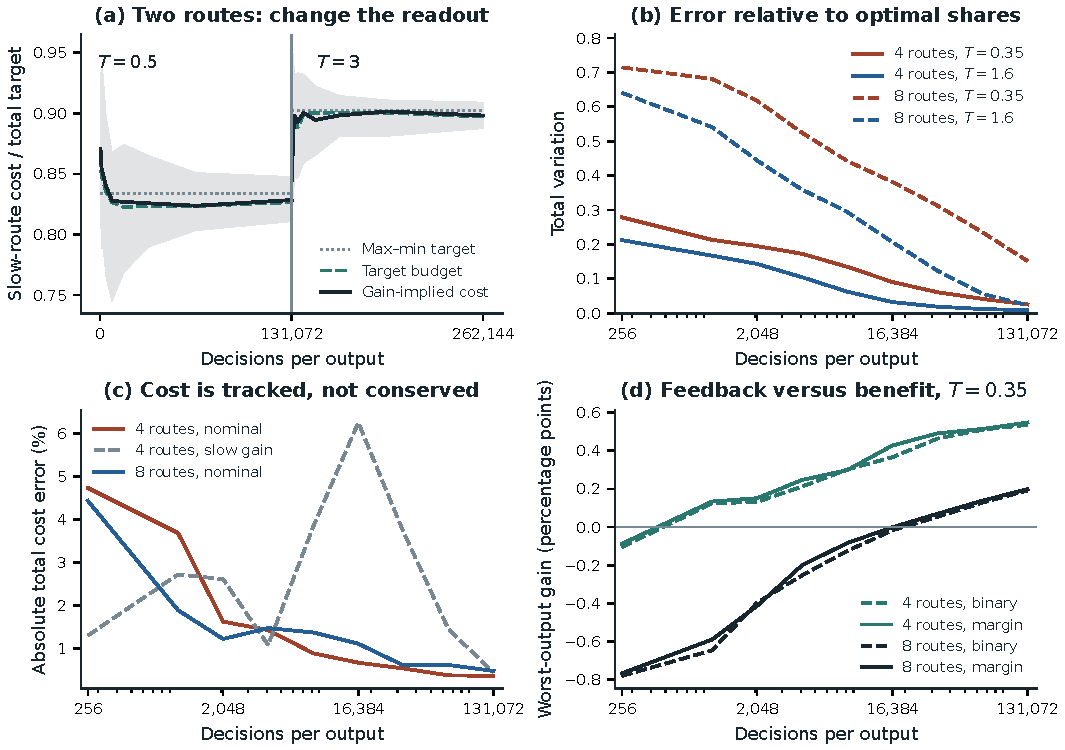
\includegraphics[width=\textwidth]{figures/fig_prrS_local_gain_loop.pdf}
\caption{\textbf{Activity-based gain regulation can follow a changing
readout, with finite-time allocation and cost errors.}
(a) In the two-route model, margin feedback redistributes the budget
after the window switch. Dotted gray shows the analytic optimum;
dashed teal shows target budget; solid dark shows frozen-gain cost.
The band is the 10th--90th percentile range across 48 realizations.
(b) Total variation from the optimal shares after normalizing the
gain-implied costs to sum to one. Solid: four routes; dashed: eight;
rust: short window; blue: long window. (c) Absolute error of the
gain-implied total cost relative to \(B\) at the short window. The
dashed gray curve uses a 64-fold slower actuator. (d) Change in
worst-output correctness evaluated at frozen gains, relative to the
unit-gain start. Dashed curves use binary feedback, solid curves
use cue-aligned margins. All curves are medians; each checkpoint
evaluates the second-half average of its run prefix.}
\label{fig:localgainloop}
\end{figure}

The model assigns functions to possible regulatory components:
neighbor comparisons transfer a conserved target resource and the
local filter tracks how strongly input fluctuations drive an output.
It assumes access to cue-free or separated source-driven activity,
evaluable task feedback, and a forward gain actuator that does not
modify the recurrent dynamics. It does not identify a biological
circuit that computes these quantities or maintains this resource.

\FloatBarrier
\section*{Data and code}
The datasets are available from their cited public releases. The source
repository is \url{https://github.com/Mia9469/SSNN}. The source package
accompanies this manuscript and includes the analysis code,
machine-readable results and instructions; third-party recordings and
connectome tables are not redistributed.

\bibliographystyle{apsrev4-2}
\bibliography{references,references_prr}
\end{document}
